\documentclass[11pt,fleqn]{article}

% For figures
\usepackage{graphicx}
\usepackage{ifpdf}

% For hyperlinks in PDF and HTML
\usepackage{hyperref}

% package HTML requires Latex2HTML to be installed for html.sty
\usepackage{html}
\newcommand{\doi}[1]{doi:\href{http://dx.doi.org/#1}{#1}}
\newcommand{\http}[1]{\href{#1}{#1}}
\begin{htmlonly}
\renewcommand{\href}[2]{\htmladdnormallink{#2}{#1}}
\end{htmlonly}
\hypersetup{colorlinks,
            %citecolor=black,
            %filecolor=black,
            %linkcolor=black,
            %urlcolor=black,
            bookmarksopen=true,
            pdftex}
 
\addtolength{\textwidth}{1.0in}
\addtolength{\oddsidemargin}{-0.5in}
\addtolength{\topmargin}{-0.5in}
\addtolength{\textheight}{1.0in}
\newcommand{\re}{\mbox{$r_{e}$}}
\newcommand{\nico}{\mbox{Ni(CO)$_{4}$}}
\newcommand{\crno}{\mbox{Cr(NO)$_{4}$}}
\newcommand{\feco}{\mbox{Fe(CO)$_{5}$}}
\newcommand{\mncoh}{\mbox{Mn(CO)$_{5}$H}}
\newcommand{\pyridine}{\mbox{C$_{5}$H$_{5}$N}}
\newcommand{\siosit}{\mbox{Si$_{8}$O$_{7}$H$_{18}$}}
\newcommand{\siosifo}{\mbox{Si$_{8}$O$_{25}$H$_{18}$}}
\newcommand{\siosifi}{\mbox{Si$_{26}$O$_{37}$H$_{36}$}}
\newcommand{\siosis}{\mbox{Si$_{28}$O$_{67}$H$_{30}$}}

\pagestyle{headings}
\pagenumbering{roman}
\begin{document}
\sf
\parindent 0cm
\parskip 1ex
\begin{flushleft}
 
Computing for Science (CFS) Ltd.,\\CCLRC Daresbury Laboratory.\\[0.30in]
{\large Generalised Atomic and Molecular Electronic Structure System }\\[.2in]
\rule{150mm}{3mm}\\
\vspace{.2in}
{\huge G~A~M~E~S~S~-~U~K}\\[.3in]
{\huge USER'S GUIDE~~and}\\[.2in]
{\huge REFERENCE MANUAL}\\[0.2in]
{\huge Version 8.0~~~June 2008}\\ [.2in]
{\large PART 14. THE PARALLEL IMPLEMENTATION}\\
{\large MPP, SMP and Commodity-based Systems}\\
\vspace{.1in}
{\large M.F. Guest, P. Sherwood, H.J.J van Dam, I.J. Bush and J.M.H. Thomas}\\[0.2in]
 
Copyright (c) 1993-2008 Computing for Science Ltd.\\[.1in]
This document may be freely reproduced provided that it is reproduced\\
unaltered and in its entirety.\\
\vspace{.2in}
\rule{150mm}{3mm}\\
\end{flushleft}

\tableofcontents

\pagenumbering{arabic}

\newpage

\section{Introduction}

In this chapter we describe the specific features and directives of
the parallel versions of GAMESS-UK, with details on executing the code
on MPP machines, such as the IBM p-series systems, 32- and 64-bit
Linux platforms, and on SMP systems such as the Silicon Graphics Altix
and Cray XD family. Familiarity with the serial version is
assumed, and these notes should be read in conjunction with the
previous parts of the User's Guide and Reference Manual.

\subsection{Background and structure of the parallel code}

Historically there were two different parallel versions of GAMESS-UK
that were maintained as separate binaries. The different versions have
now been combined into a single binary, and the functionality is now
available as different drivers (or modules) within this binary.

The different parallel drivers are:

\begin{itemize}
\item A replicated data driver that relies on the virtual shared
  memory model provided by the Global Array toolkit (the ''GA
  driver'').
\item A (predominantly) distributed-data driver that is parallelised
  using MPI and makes use of MPI-based tools such as BLACS and
  ScaLAPACK (the ''New SCF driver'').
\end{itemize}

Although they co-exist in a single binary, the different drivers make
use of different communication libraries and parallel toolkits. Figure
1 shows how these various technologies relate to each other and the
interconnect on the machine.

\begin{figure}[h]
\centering
\ifpdf
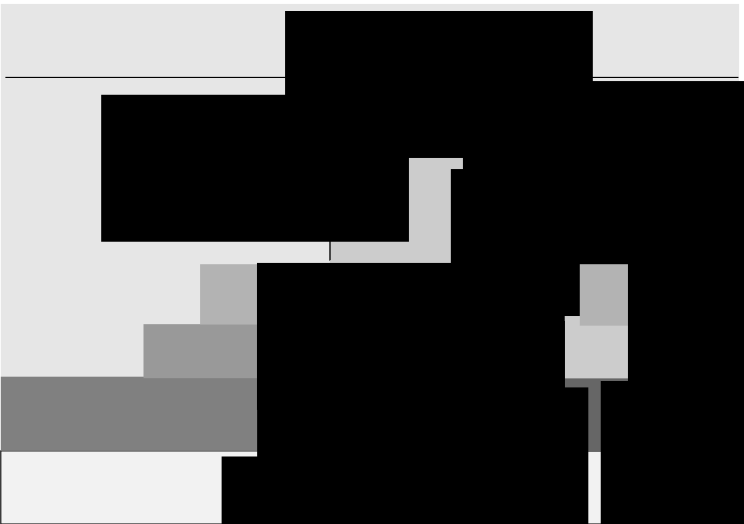
\includegraphics[scale=0.5]{p14_fig1.pdf} \\
\else
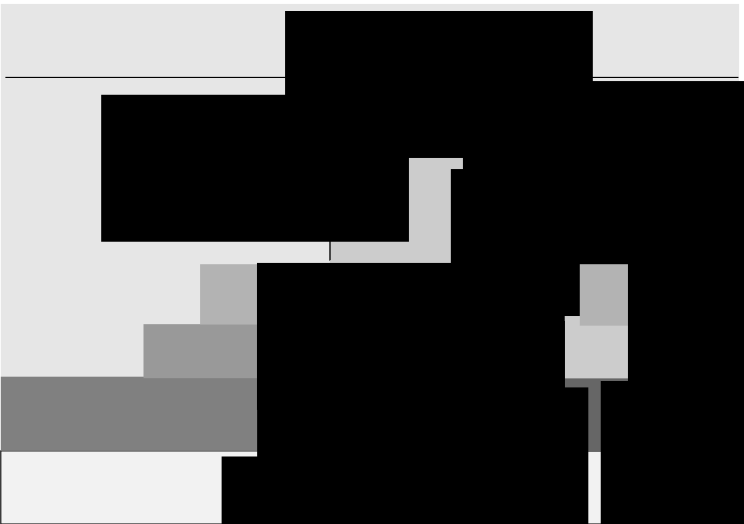
\includegraphics[scale=0.5]{p14_fig1.eps} \\
\fi
\caption{The different parallel drivers.}
\end{figure}

If neither the GAs or ScaLAPACK are available, a parallel version of
GAMESS-UK may still be compiled. This version effectively exposes the
simple underlying parallel code that is built on and extended by the
two drivers mentioned above. This code is described in the section on
the ``Simple MPI Driver''.

The following sections briefly describe the genesis and strucuture of
the different drivers.

\subsubsection{The Global Array (GA) driver}
The GA driver has been parallelised using a number of the tools
developed by the High Performance Computational Chemistry Group
(HPCCG) from the Environmental Molecular Sciences Laboratory at PNNL.

The first of these is the Global Array (GA) toolkit \cite{GA1,GA2,GA3}, which
provides an efficient and portable 'shared-memory' programming
interface for distributed memory computers. The toolkit enables each
process in a MIMD parallel program to asynchronously access logical
blocks of physically distributed matrices, without need for explicit
co-operation by other processes. Unlike other shared-memory
environments, the GA model exposes the programmer to the non-uniform
memory access (NUMA) timing characteristics of the parallel computers
and acknowledges that access to remote data is slower than to local
data.

The GA's can be built on top of a number of different communication
technlogies. In order to support one-sided communications, the GA's
make use of the ARMCI library. A simple and portable version of ARMCI
can be built on top of a standard sockets library, although in some
cases optimised versions of ARMCI are available that have been ported
directly to the interconnect on the machine.

For the two-sided communications, the GA's are usually configured to
use the MPI library on the machine. The GA's may be configured to use
the TCGMSG message passing library (which in turn may built on top of
MPI or using sockets), but this is not recommended for most users; the
only likely exception is for users who require to build the entire
code with 64-bit integers (i8). This may be required for running
exceptionally large calculations where the indexes into arrays are
likely to overflow a 32-bit integer.

The GAs also provide an interface to libraries for solving eigenvalue
equations. The default library is PeIGS (described below), as the
source code is supplied with GAMESS-UK and is therefore guaranteed to
be present. The GAs may also be configured to use the ScaLAPACK
library if one is available on the machine. If ScaLAPACK is availble,
we would recommend making use of it (by configuring the code with the
``scalapack'' keyword), as it should lead to an increase in
performance of the GA code. In addition, using ScaLAPACK will also
significantly improve the performance of the New SCF driver.

\textbf{PeIGS}\\
PeIGS is the scalable, fully parallel eigensolver whose numerical
properties satisfy the needs of the chemistry applications
\cite{PEIGS1}. PeIGS solves dense real symmetric standard (Ax = lx)
and generalized (Ax = lBx) eigenproblems. The numerical method used is
multisection for eigenvalues and repeated inverse iteration and
orthogonalization for eigenvectors \cite{PEIGS1}. Accuracy and
orthogonality are similar to LAPACK’s DSPGV and DSPEV
\cite{LAPACK1,LAPACK2}. Unlike other parallel inverse iteration
eigensolvers, PeIGS guarantees orthogonality of eigenvectors even for
arbitrarily large clusters that span processors. Internally, PeIGS
uses a conventional message passing programming model and
column-distributed matrices. However, it is more commonly accessed
through an interface provided by the GA toolkit, with the necessary
data reorganization handled by the interface.

Once the capability for GA is added to GAMESSUK, and the PeIGS- or
ScaLAPACK-based diagonalization module introduced, parallelization of
the linear algebra becomes straightforward by forming a distributed
copy of the relevant matrices and calling the library routine.
Depending on the subsequent operation, it may then be necessary to
re-replicate the array. As an example, the SCF convergence
acceleration algorithm (DIIS - direct inversion in the iterative
subspace) uses GA storage for all matrices, and parallel matrix
multiply and dot-product functions. This not only reduces the time to
perform the step, but the use of distributed memory storage (instead
of disk) reduces the need for I/O. We have also used the GA tools to
map disk files into distributed memory, an approach which proves more
efficient than keeping all files on node 0 and distributing to all
nodes using broadcast operations.

The following functionality is available within the GA driver.

\begin{itemize}
\item RHF, ROHF, UHF and GVB energies and gradients (conventional, in-core
and direct), including effective core potentials.
\item Direct-MP2 energies and gradients (closed-shell).
\item Direct-SCF analytic 2nd derivatives.
\item Solvation using the Tomasi Polarizable Continuum Model.
\item Direct RPA.
\item Analysis options requiring the computation of properties on
      molecular grids.
\item Density Functional Theory (DFT):
  \begin{itemize}
  \item closed- and open-shell (UKS) energies and
    gradients, with both explicit and fitting treatments of the Coulomb
    term.
  \item Analytic Second Derivatives
  \end{itemize}
\item Valence Bond module
\item Zeroth Order Regular Approximation (ZORA)
\item Direct Configuration Interaction (CI) (although this code
  requires the presence of a parallel filesystem, accessible by all
  nodes on the system).
\end{itemize}


\subsubsection{The New SCF driver}

This SCF/DFT driver, using MPI-based tools such as BLACS and
ScaLAPACK, was originally developed to overcome problems with scaling
on the IBM p-series system HPCx running with SP7, and also to address
problems related to the largest chemical system that would fit in to
the available memory with the replicated data GA version.

In the light of these problems an approach was investigated, in which: 

\begin{itemize}
\item MPI-based tools (such as ScaLAPACK) were used in place
of GA and LAPI
\item all data structures except those required for the Fock matrix
  build were fully distributed.
\end{itemize}

A partially distributed model was chosen because, in the absence of
efficient one-sided communications, it is difficult to efficiently
load balance a distributed Fock matrix build. The obvious drawback of
this is that some large replicated data structures are
required. However, these are kept to a minimum. For a closed shell
Hartree-Fock or density functional theory calculation only two
replicated matrices are required, one Fock and one density, while for
unrestricted calculations this is doubled. Further, the symmetry of
these matrices is used to cut down on the required memory.

The ScaLAPACK SCF module is written in standard conforming Fortran 95,
and uses MPI for message passing. The code is built upon a Fortran
module that implements a derived matrix type and operations on such
objects, the defined operations being those commonly use in quantum
chemistry. The matrices can be either replicated or distributed, this
being set when they are created. After that the routines that use the
module need not know how a given matrix is distributed, thus
simplifying the high level implementation. For distributed matrices
the matrix operations are, in general, performed using ScaLAPACK
\cite{SCALAPACK1,SCALAPACK2}, while LAPACK \cite{LAPACK1,LAPACK2} is
used for replicated matrices. Using multiple BLACS \cite{BLACS1}
contexts allows linear algebra operations to be performed on a subset
of the processors, and this is exploited by the matrix module to use
the extra level of parallelism available in unrestricted calculations,
i.e. that over the spins. These underlying distributed operations are
transparent to the high level routines. This is achieved by
overloading many of the operations on the matrix type, allowing them
to act on both single matrices and arrays of them.

The following functionality is currently available within the
ScaLAPACK driver:

\begin{itemize}
\item RHF and UHF (but not ROHF) energies and gradients.
\item Closed and open-shell DFT energies and gradients.
\end{itemize}


\subsubsection{Simple MPI driver}
If ScaLAPACK and the GAs are unavailable, an MPI version of the code
may still be compiled and the default SCF/DFT driver is then the one
described below.

This driver is only of interest for systems where the GA code, as well
as BLACS and ScaLAPACK are unavailable. It may also occasionally be of
use on dual-processor workstations, for example, where the memory
requirements of the GA and ScaLAPACK versions would be too great, but
a speedup would be gained by splitting some of the work across both
processors.

This code resulted from both SCF and DFT modules being parallelized in
replicated data fashion, with each node maintaining a copy of all data
structures present in the serial version. While this structure limits
the treatment of molecular systems beyond a certain size, experience
suggests that it is possible on the current generation of machines to
handle systems of up to 5000 basis functions. The main source of
parallelism in the SCF module is the computation of the one- and
two-electron integrals and their summation into the Fock matrix, with
the more costly two-electron quantities allocated dynamically using a
shared global counter. The result of parallelism implemented at this
level is a code scalable to a modest number of processors (around 32),
at which point the cost of other components of the SCF procedure start
to become significant.

The following functionality is available within this implementation:

\begin{itemize}
\item RHF, ROHF and UHF energies and gradients.
\item Closed and open-shell DFT energies and gradients.
\end{itemize}


%% \subsubsection{GAMESS-UK Taskfarming binary}

%% A taskfarming capability for GAMESS-UK has been developed that allows
%% a user to batch process multiple small jobs on a subset of the total
%% number of processors allocated to GAMESS-UK on a large parallel
%% machine.

%% The taskfarm reserves one processor as ''server'' process and then
%% splits the remaining processors into groups of a user-defined size,
%% with any left-over processors forming an additional group that will be
%% of a different size to the others, but used in an identical fashion.

%% The server process then reads in a list of the jobs to run, and
%% allocates each group a job. As a group finishes running a job, it will
%% contact the server to state it has finished, whereupon the server will
%% allocate it a new job if there are still any outstanding.

%% The taskfarm ends when there are either no more jobs to process or a
%% user-defined percentage of the groups are sitting idle.

%% The taskfarm capability is compiled as a separate binary by
%% configuring the code with the ``taskfarm'' keyword.

%% This functionality is incomplete and experimental, so users should
%% contact the GAMESS-UK support team if they are intersted in using this
%% functionality.

%% \subsection{Availability}

%% GAMESS-UK can be made to run on almost any parallel platform. A list
%% of the currently supported ports as of the writing of this manual is
%% below, but new ports are always being added and additional ones can be
%% added on request if the developers can be provided with access to the
%% system.

%% \begin{itemize}

%% \item Pentium- and Athlon-based Linux systems
%% \begin{itemize}
%% \item available for MPICH (Intel and PGI compilers) and SCORE systems (Intel compilers)
%% \end{itemize}

%% \item EM64T-based Linux systems
%% \begin{itemize}
%% \item available for MPICH (Intel compilers)
%% \end{itemize}

%% \item Itanium-based Linux systems
%% \begin{itemize}
%% \item available for MPICH (Intel compilers)
%% \end{itemize}

%% \item Opteron-based Linux systems
%% \begin{itemize}
%% \item available for MPICH systems running over Myrinet (PGI compilers)
%% \item available for SCORE systems (Intel compilers)
%% \end{itemize}

%% \item IBM PowerPC (3, 4 \& 5)-based AIX systems
%% \begin{itemize}
%% \item available for MPI over LAPI (XLF compiler)
%% \end{itemize}

%% \item SGI systems
%% \begin{itemize}
%% \item available for Altix systems running over the SGI MPI
%%   implementation (Intel compilers)
%% \item available for Origin systems running over MPI (MIPSpro compiler)
%% \end{itemize}

%% \item HP-UX systems 
%% \begin{itemize}
%% \item available for Itanimum 2 processors running over HP's MPI implementation (HP F90 compiler)
%% \end{itemize}

%% \end{itemize}

\subsection{Differences from the Serial Code}

Users of the parallel code should be aware of a number of
significant differences with respect to the serial version. These will
affect the way the program is executed, and (to a lesser extent) may
affect the input directives employed.

\begin{enumerate}

\item The compilation and execution of the code may be influenced by
  the parallel tools used, including the parallel harness (MPI,TCGMSG),
  the MPI implentation, the Global Array (GA) Tools and the parallel
  diagonaliser (PeIGS) and MPI-based tools such as BLACS and ScaLAPACK.

\item The weakness (and diversity) of I/O performance on parallel
  machines leads to various I/O options for the GA-based code,
  including the use of replicated files (one for each node). This has
  implications for file naming.  On some machines the direct-SCF is to
  be strongly preferred to the conventional SCF mode.

\item Some adjustments to the input may be needed to get the best
  performance e.g., the load-balancing strategy may be adjusted, or
  certain parallel segments of code activated or deactivated.

\end{enumerate}

\section{Building and running the parallel version of GAMESS-UK}

\subsection{Configuring the parallel version}

The parallel version of the code is configured by selecting the
''parallel'' option (from the serial and parallel options offered)
when running the configure script.

Once you have selected the compiler that you would like to use, you
will be presented with a series of options similar to that shown
below:

{
\footnotesize
\begin{verbatim}

 Using include file:  /home/jmht/GAMESS-UK/config/x86_64-unknown-linux-gnu-parallel-pgi.mk

The recommended (default) options for this build are:
 ga mpi mp2 peigs newscf dl-find zora vb vdw masscf mpiwrap

 In addition, the following options are available:
 score blas myrinet datain i8 scalapack

 Please enter any additional options from the list above that you would
 like to include in this build or just hit enter to go with the defaults.
 NB: to remove default options, prefix them with a minus sign.

\end{verbatim}
}

In most cases, you should just run with the default options. The only
options you are likely to want to change are the addition of the
''scalapack'' or ''blas'' options if you have ScaLAPACK or optimised
blas libraries available on your machine, or the addition of the
option for your interconnect (e.g. ''myrinet'' above).

If you are running very large calculations and know that you need to
run in ''i8'' mode (64bit FORTRAN integers), then you cannot currently
also use the scalapack option, as this is only available with 32-bit
integers.

To build the ''simple MPI'' driver, you need to choose a base build
and remove the ga and peigs options, together with all the extra code
modules that require the Global Arrays to function (ci, mp2, zora, vb
and masscf). In the above case, you would type in the following at the
prompt to achieve this:


{
\footnotesize
\begin{verbatim}

-ga -peigs -mp2 -zora -vb -masscf base

\end{verbatim}
}


\subsection{Running the parallel version}
For the parallel code, a binary named ''gamess-uk'' will be created in
the directory:

{
\footnotesize
\begin{verbatim}
          GAMESS-UK/bin
\end{verbatim}
}

If rungamess script has been configured correctly (see chapter 13 for details
on the rungamess), this may be used to run the code.

Otherwise, the binary should be run as any other parallel code, using
a command such as mpirun or poe, with the input being piped to the
binary as shown below:

{
\footnotesize
\begin{verbatim}
  /usr/bin/mpirun -np 32 /home/fred/GAMESS-UK/bin/gamess-uk < input.in > ouput.out
\end{verbatim}
}

\subsubsection{DATAIN and broken MPI-implementations}
Some MPI implementations suffer from a problem that the input buffer
is of limited size and piping large input files to GAMESS-UK may cause
the code to hang. To work around this problem, the program may be
configured with the ''datain'' keyword.

Use of this keyword causes GAMESS-UK to look for its input from a
file called ''datain'' that should be found in the directory where the
job is running from.

In those cases, the following steps would then be required to run the job:

{
\footnotesize
\begin{verbatim}
  cp input.in datain
  /usr/bin/mpirun -np 32 /home/fred/GAMESS-UKbin/gamess-uk  > ouput.out
\end{verbatim}
}


%% \subsection{Running the tcgmsg version}
%% If the code has been built without MPI, then a binary called
%% ''parallel'' will be created in the GAMESS-UK/bin directory.

%% The binary 'parallel' is then used to execute GAMESS-UK. It needs to
%% read a configuration file to determine which process to run where. The
%% configuration file consists of one or more data lines containing the
%% following white space separated data fields:

%% {
%% \footnotesize
%% \begin{verbatim}
%%         <userid>  <hostname>  <nproc>  <executable>  <workdir>
%% \end{verbatim}
%% }
%% where
%% \begin{itemize}
%% \item {\em userid} is the username on the machine that will be
%% executing the process.

%% \item {\em hostname} is the hostname of the machine on which to execute
%% the processes.  The name must match the value returned by the command
%% ``hostname''. Note that the user must ensure that the job is not
%% redirected to a different host by ensuring that the -m parameter, if
%% specified, is consistent with <hostname>.

%% \item {\em nproc}  is the total number of copies of this process to be
%% executed on the machine, where each process is using shared memory to
%% communicate.

%% \item {\em executable} is the full path name of the GAMESS-UK
%% executable i.e. 
 
%% {
%% \footnotesize
%% \begin{verbatim}
%%           /home/fred/GAMESS-UK/bin/gamess-uk
%% \end{verbatim}
%% } 

%% \item {\em workdir} is the full path name on the machine of the
%% directory to work in.  If specified as a ``.'' then processes will use
%% the current directory from which the job was submitted.
%% \end{itemize}

%% The configuration file should be named with a .p suffix
%% (e.g. ''myconfig.p''), and the parallel binary should then be invoked with
%% the first argument being the name of the configuration file, minus the
%% suffix (i.e. ''myconfig'').

%% The parallel program uses rsh or ssh to communicate with the different
%% nodes. By default, the program will try and use /usr/bin/rsh, although
%% this can be changed by setting the environment variable ''TCGRSH'' to
%% contain the path to the relevant rsh/ssh binary.

%% \textbf{NB:} You will be required to enable passwordless rsh/ssh
%% access between the nodes, for example by using ssh public/private
%% keys.

%% For example, to use the /usr/bin/ssh binary you would use the
%% following command under a Bourne shell (sh/bash/ksh):

%% {
%% \footnotesize
%% \begin{verbatim}
%%           TCGRSH=/usr/bin/ssh; export TCGRSH
%% \end{verbatim}
%% } 

%% Or the following under a C-type shell (csh/tcsh):

%% {
%% \footnotesize
%% \begin{verbatim}
%%           setenv TCGRSH /usr/bin/ssh
%% \end{verbatim}
%% } 


%% {\bf Example 1}\\

%% Assuming user "gamess" wishes to execute a 4 processor job on the
%% machines called king.sara.nl and kong.sara.nl (2 processors per
%% machine), with all temporary files to be routed to the scratch
%% directory, /tmp/gamess (this directory, and the directory containing
%% the binary being accessible from both machines (via nfs, for example),
%% then the configuration file myconfig.p would comprise the two lines:

%% {
%% \footnotesize
%% \begin{verbatim}
%%   gamess king.sara.nl 2 /home/fred/GAMESS-UK/bin/gamess-uk /tmp/gamess
%%   gamess kong.sara.nl 2 /home/fred/GAMESS-UK/bin/gamess-uk /tmp/gamess
%% \end{verbatim}
%% }

%% The job may be submitted directly with file input.in containing the
%% input and output.out the resulting output, thus

%% {
%% \footnotesize
%% \begin{verbatim}
%%    /home/fred/GAMESS-UK/bin/parallel myconfig < input.in > output.out
%% \end{verbatim}
%% }


\section{Directives Common to all parallel versions of the code}

The following pre-directives, while not specific to the parallel
code are described here for completeness.

\subsection{The TIME Pre-directive}

The TIME card sets the cpu time limit for the job, e.g.
{
\footnotesize
\begin{verbatim}
        TIME 120
\end{verbatim}
}
will allocate 120 minutes of CPU time for the job. The current default
TIME allocation is 600 minutes.

\subsection{The FILE Pre-directive}

Like on other UNIX-based systems, the names used for the GAMESS-UK files
may be specified in two ways.
\begin{enumerate}
\item By setting environment variables
\item By including FILE pre-directives (see the section on pre-directives in
      chapter 3)
\end{enumerate}
The latter is more flexible, as it also allows the attributes of
the file to be modified. This is particularly relevant for parallel runs
where these attributes can be used to control the way files are stored. See 
section~\ref{pio} for a detailed discussion.

An example of defining file names with environment variables is
(assuming the use of (t)csh)
{
\footnotesize
\begin{verbatim}
          setenv ed3 test.ed3 
\end{verbatim}
}
which specifies that GAMESS-UK is to write the contents of ed3 to a file
named "test.ed3".

The FILE pre-directive that has the same effect reads
{
\footnotesize
\begin{verbatim}
          FILE ed3 test.ed3 KEEP
\end{verbatim}
}
The option KEEP is required to retain the file "test.ed3" after the job has 
finished, by default all data files are deleted at the end of the job.


\subsection{Restarting the Parallel Code}

A somewhat restricted level of restart capability is possible within
the present parallel implementation compared to the serial code.  Given
that the Dumpfile has been retained, the user may safely assume that it
is now possible to restart jobs involving geometry optimisation (under
"optimise" and "optxyz" control) and force constant evaluation
("force"). Note that the granularity of restart is, however, reduced
compared to the serial code. Assuming, for example, that an
optimisation or force constant dumps on time during the evaluation of
he gradient for a given point, the restart job will involve having to
recompute the energy of that point. This should not require any change
to the standard data presented in such cases, with the flow of tasks
controlled by the program. Thus assuming the following input file had
been presented in a direct-MP2 force constant startup job:

{
\footnotesize
\begin{verbatim}
          TIME 15
          TITLE
          SCF3 - BASIS II MP2 - ENERGY = -1059.4057998
          ZMAT ANGSTROM
          SC
          X 1 1.0
          F 1 SCF 2 90.0
          F1 1 SCF 2 90.0 3 120.0
          F1 1 SCF 2 90.0 3 -120.0
          VARIABLES
          SCF 1.8661788 HESS     .803548
          END
          BASIS
          TZVP SC
          DZP F
          DZP F1
          END
          RUNTYPE FORCE
          SCFTYPE DIRECT MP2
          LEVEL 2
          ENTER
\end{verbatim}
}
then the following data set should be presented in all subsequent
restarts of the computation:
{
\footnotesize
\begin{verbatim}
          TIME 30
          RESTART FORCE
          TITLE
          SCF3 - BASIS II MP2 - ENERGY = -1059.4057998
          PUNCH COORDINATES BASIS
          ZMAT ANGSTROM
          SC
          X 1 1.0
          F 1 SCF 2 90.0
          F1 1 SCF 2 90.0 3 120.0
          F1 1 SCF 2 90.0 3 -120.0
          VARIABLES
          SCF 1.8661788 HESS     .803548
          END
          BASIS
          TZVP SC
          DZP F
          DZP F1
          END
          RUNTYPE FORCE
          SCFTYPE DIRECT MP2
          LEVEL 2
          ENTER
\end{verbatim}
}


\section{Directives specific to the GA version of the code}

\subsection{Overview}

This section describes the main features of the Global Array-based code that may
require specific attention by the user.  Most of the time we hope the
defaults will provide reasonable performance.  The majority of these
features are controlled by the new PARALLEL directive, but there
are changes, in particular other options to the FILE
pre-directive. Note also that these options are not consistently
available across all parallel machines; we draw attention to such
machine dependencies in the notes below.

\subsection{Memory Allocation - The MEMORY predirective}

The parallel code for MPP machines makes use of the Global Array (GA)
tools from Pacific Northwest National Lab \cite{GA1}  for the allocation
and manipulation of distributed data structures. The memory assigned to
these arrays, subsequently referred to as the MA memory,  is shared
across the MPP machine; the GA tools allow any node to read or write
to any part of the data structure without synchronisation.

An important side-effect is that a memory segment has to be set aside
for the global arrays. We have now made the internal memory allocation
scheme within GAMESS-UK consistent with this requirement, with the
standard MEMORY pre-directive allocating the total memory
(covering the two memory segments, one for use by the GA's and those
sections of the code that have been converted to share this memory, and
one for the remaining segments).

The total memory is allocated using the directive:
\label{mamem}
{
\footnotesize
\begin{verbatim}
          MEMORY 3500000
\end{verbatim}
}
The effect of this directive will be to specify the amount of memory
{\em per node} to be allocated toward the total available for the
job. Thus on an 8-node configuration the above directive will result in
a total memory of 28 MWords; on a 32-node configuration the effect
will be to realise 112 MWords. From this it is evident that errors
attributed to too small a global allocation can be circumvented by
increasing the number of nodes assigned to the task in hand.

The default node memory allocation is usually 20 Mwords, but is
may be different depending on the architechture. These
allocations are appropriate for installations with 256 MByte memory
nodes, and may not be appropriate for machines with differing node
memories. Suggested memory allocations for machines with 64, 128 and
512 MByte memory nodes are 4, 10 and 48 Mwords respectively.

The allocation that has been used for a job is printed towards the
beginning of the GAMESS-UK output, with a line similar to the below:

{\footnotesize
\begin{verbatim}
          main store requested   5000000 real*8  words
\end{verbatim}
}

Indicating that 5 million words (40Mbytes) were requested.

\subsection{Parallel I/O Options}
\label{pio}

I/O on many parallel MPP machines is poor by comparison with the CPU
performance, so the optimum strategy will be a function of the parallel
architecture, the hardware configuration, and the number of nodes
used.  A number of options are provided to control the I/O activity,
both for individual files and to control the strategy adopted by the
code as a whole.  Consider first the following ways in which I/O to a
particular file may be handled:

\begin{enumerate}
\item \label{indi} Each node maintains an independent copy of the file:
\item \label{distrib} Each node holds a partial copy (and only reads/writes a
subset of the information);
\item \label{node0} Node 0 manages a copy of the file and message-passing is
used to distribute data to the other nodes;
\item \label{incore} Each node holds the whole file in memory;
\item Each node holds part of the file in memory  (and only accesses a subset
   of the information);
\item \label{gafs} Each node holds part of the file in memory, but may write or
access data held on other nodes.
\end{enumerate}

Options \ref{indi} and \ref{incore} correspond to the normal serial
execution with disk or memory specifications. As the parallel version
of GAMESS-UK basically works on a replicated model (all nodes execute
the whole code and store all the data) these modes can also be used by
the parallel version, and may be useful for machines like the SP2
or workstation clusters where there is a local disk fitted to each
node.  However, for large numbers of nodes the disk and memory
requirements will be excessive and will prohibit scalability.

Where memory and disk resources are scarce, Option \ref{node0} is
preferable, but implies increased communications costs as the read
operation (when performed on every node) will require data to be
broadcast from node 0. Where communications are good, however, this is
a viable strategy.  A reduction in the communications costs can be
achieved if the number of reads by nodes other than node 0 can be
reduced. Often this may be accomplished by adopting a master-slave
model in which the slaves are idle during serial sections of work
(rather than performing it concurrently with node 0 (see below).

The distributed file, Option \ref{distrib} is clearly only feasible for
files used in parallel sections of the code where each node has a
distinct sub-set of the data to work with. It also requires all nodes
to have efficient I/O capabilities. The integral file in conventional
SCF calculations can be split in this way - so this option is useful
for such calculations on machines with node disk - e.g., the SP2 or
workstation clusters. Option 5 can be used similarly to map a
distributed file into distributed memory.

Option \ref{gafs} is available whenever the GA version of GAMESS-UK has
been built. A Global Array is allocated for each file to be
distributed.  This option implies even more communications than 
Option \ref{node0}, but has been implemented to maximise the size of
transfers, and on a low-latency machine is likely to be more
efficient.  It is valuable for machines with poor I/O performance but
good communications.

The I/O options may be controlled either by the PARALLEL IOMODE
pre-directive (see below) which modifies the settings for all files
used by a job, or on a file-by-file basis using the FILE
pre-directive. The former is recommended, but for completeness some of
the FILE settings that may be useful in practice are summarised
below.

\begin{enumerate}
\item {\bf Specifying the name for a file:}
{
\footnotesize
\begin{verbatim}
          FILE <stream> <filename> [ KEEP ]
\end{verbatim}
}
The KEEP keyword is added if the file is required beyond
the end of the job. Once a file directive has been specified, the
default is to delete it.
\noindent
\item {\bf Mapping a file into memory:}
{
\footnotesize
\begin{verbatim}
          FILE <stream> MEMORY LENGTH <length>
\end{verbatim}
}
\noindent
\item {\bf Mapping a file into a global array:}
{
\footnotesize
\begin{verbatim}
          FILE <stream> <filename> GAFS LENGTH <length>
\end{verbatim}
}
\end{enumerate}

\subsection{Parallel I/O Modes - The PARALLEL pre-directive}
\label{piomode}

While the I/O option for each file can be set individually, a number of
I/O modes for the code as a whole have been defined. These modify the
I/O options for certain files, as well as modifying the route through the
code to maximise efficiency. It is recommended that these are chosen rather
than adjusting individual file settings. In the following we limit discussion
to the Dumpfile (ED3), Scratchfile (ED7) and Mainfile (ED2).

The I/O mode is set by the PARALLEL IOMODE pre-directive with an
appended  keyword.  {\em e.g.}
{
\footnotesize
\begin{verbatim}
          PARALLEL IOMODE NZO
\end{verbatim}
}
Valid keywords include the following;
\begin{itemize}
\item INDIVIDUAL, or INDI - This corresponds to the default file 
       option \ref{indi}. The Mainfile, ED2, if used will have 
       option \ref{distrib}.
\item SCREENED - ED3 and ED7 will be handled using option \ref{node0},
   ED2 by option \ref{distrib}, with a master-slave algorithm adopted
   to reduce read activity on the slave nodes.  This is suitable for
   machines with poor communications (e.g., workstation clusters)
\item NZO  - ED3 and ED7 will be handled using option \ref{node0}, ED2
   by option \ref{distrib}. In contrast to the SCREENED option, 
   there will be no attempt to reduce communications
   by adopting a master-slave strategy.
\item GAFS - ED3 and ED7 will be handled using option \ref{gafs}, ED2
   by option \ref{distrib}. There will be no attempt to reduce
   communications by adopting a master-slave strategy. Note that unless
   FILE directives are also added, a default length (per node) will be
   allocated for these streams. GAFS mode is at present the default on
   the Cray T3D and T3E, IBM SP and IA-32 and Alpha Linux Clusters,
   with GAFS processing at present markedly superior on both the T3D and
   T3E compared to, say, NZO. This advantage is less marked on the SP
   and commodity clusters (given node disk capability).  In these cases
   the keyword NOGAFS can be used to switch the mode off, and should be
   presented before any FILE predirectives.

\end{itemize}

The main advantage of the NZO mode is that as all nodes are running
through the whole code, there is scope for additional parallelisation
of the linear algebra. This is likely to be useful for large problem
cases running on large MPP machines with good communications.

The NZO mode can be specified for individual files by specifying it in a file
directive or by including the string nzo in the name of the file if setenv is used.
This is needed when an ed3 file is used as say ed12 in a following job.

When files are held in GAs, premature termination of the job will cause
all data stored in them to be lost.  In the special case of a Dumpfile
which the user has requested be kept after the completion of a run,
GAMESS-UK will periodically write the contents of the GAFS to the disk
copy of the file. This currently occurs on termination of the SCF (or
on termination of each SCF in, for example, a geometry optimisation),
and at the end of each job step. As I/O operations are expensive, this
process will affect the performance of the job, and in cases where
there is little risk of the job running out of time the updating of the
file can be suppressed by appending NOUPDATE to the PARALLEL IOMODE
directive:

{
\footnotesize
\begin{verbatim}
          PARALLEL IOMODE GAFS NOUPDATE
\end{verbatim}
}
Presenting the data line:
{
\footnotesize
\begin{verbatim}
          PARALLEL IOMODE GAFS UPDATE
\end{verbatim}
}
provides a more regular update to disk, with the disk copy of the GAFS
updated at the end of each SCF iteration, and at the end of each job step.
Finally, the user should note that when files are to held in the GAs,
the program will allocate a certain amount of memory per node to the
total space required to store each memory-mapped file. It is quite
possible that this default allocation (e.g. 1000 blocks per node on the
T3D and IBM SP2/TN2, and 3000 per node on the Cray T3E, IBM SP/P2SC,
SP/WH2-375 and SP/p690 and commodity clusters) will prove insufficient,
particularly when running large basis function calculations on a small
number of nodes; in such cases the job will abort with an error message
typified by the following:

{
\footnotesize
\begin{verbatim}
    WRT3: Insufficient space in Global arrays
    GAMESS-UK Error on node  24: WRT3: Insufficient space in Global arrays
\end{verbatim}
}
Following the syntax given above, the user may overwrite this default
allocation.\\

{\bf Example:} The following data lines may be used to allocate
70,000 blocks to ED3 and 50,000 blocks to ED7; typically such
figures will have been derived from a successfully completed
job (see below) and will be used to define the gafs requirement
when running the corresponding job on a smaller number of nodes.

{
\footnotesize
\begin{verbatim}
          FILE ED3 MFGED3 GAFS LENGTH 70000 DELETE
          FILE ED7 MFGED7 GAFS LENGTH 50000 DELETE
\end{verbatim}
}
On the T3E, with 3000 blocks allocated per node, we see that a 64-node
job, allocating 64 X 3000 i.e 192,000 blocks in default would have been
adequate for this job. Node that the code partitions the available GA
space equally between ED3 and ED7 i.e. 96,000 blocks to each.
Attempting to conduct the calculation on 32 nodes would have led to an
error condition; the 48,000 blocks allocated to ED3 and to ED7 would
not have been sufficient for either data set.  The following points
should be noted:
\begin{itemize}
\item The appearance of the DELETE keyword as the final keyword
on the FILE directives means that the GAfs will {\em not} be saved
on job completion, and will prevent the periodic updating of the
file that will limit the efficiency of parallel execution.
\item The total space actually used by each of the GAfs is given
on job completion through the following output:

{
\footnotesize
\begin{verbatim}
           GAfs high water mark summary:
           Unit     Max blocks
            3        44147
            7        24757
\end{verbatim}
}
\item Note that in contrast to the serial code, the parallel version
will not, when operating in default RUNTYPE mode i.e. a simple scf
calculation, generate a number of the sections that would typically be
used by subsequent RUNTYPEs, hence minimising the space requirements of
the file. This strategy is only in effect in parallel SCF calculations,
and is not used with RUNTYPEs such as "optimize".
\item Typical lengths of ED3 and ED7 (in blocks) as a function of number of
      basis functions are shown below:\\

\begin{centering}
\begin{tabular}{| c | c | c |}
\hline \hline
Number of       & Length of & Length of   \\
Basis Functions & ED3       & ED7          \\ \hline
    166         &  556      &     390     \\
    410         &  2875     &    1814     \\
    480         &  4407     &    3164     \\
    543         &  5621     &    4060     \\
    882         &  14399    &   10680     \\  
   1000         &  18489    &   13718     \\  
   1350         &  33097    &   24990      \\
   1620         &  47516    &   35980     \\ \hline \hline
\end{tabular}

\end{centering}

\end{itemize}


\subsection{Directory Specification}

It is possible to specify a default directory for the routing of files,
which will be applied to all files with names that do not begin with /.

{
\footnotesize
\begin{verbatim}
          DIRECTORY <direc>
\end{verbatim}
}

\subsection{Diagnostic output}
{
\footnotesize
\begin{verbatim}
          PARALLEL PRINT ALL
\end{verbatim}
}

Will give timing information for all nodes (rather than just the root node).

\subsection{Dynamic Load Balancing}

The PARALLEL CHUNK pre-directive is used to control load
balancing. Several sections of the code have parallelised nested loops
(e.g. the two electron integrals). The ``chunk factor'' is the number of
loop indices comprising a task assigned dynamically to a node.
It may be controlled in two ways:

{
\footnotesize
\begin{verbatim}
          PARALLEL CHUNK TASK <n>
\end{verbatim}
}
the chunk size is computed so that there will be a total of
$<$n$>$ tasks per node.  This is the default algorithm (with $<$n$>$=40).

{
\footnotesize
\begin{verbatim}
          PARALLEL CHUNK LIMIT <n>
\end{verbatim}
}
It is unlikely that the user will need to consider resetting the 
default options.

\subsection{Parallel linear algebra}

The GA version of GAMESS-UK contains parallel implementations of some
of the linear-algebra components of the SCF. The cost of performing
these steps serially is insignificant for small numbers of processors,
(they scale as O(N$^3$), N = the number of basis functions), but for
large problems ($>$ 500 basis functions) on large MPP machines ($>$ 64
nodes) they significantly inhibit scaling.

By default, the parallel linear algebra capabilities are active for
matrices of dimension $>$ 200, but this can be modified with the
following  PARALLEL pre-directives. The matrix size in these
directives may be replaced by the character string NEVER to request 
that the parallel routines are never invoked.
\begin{itemize}
\item The parallel diis solver may be controlled by the data line
{
\footnotesize
\begin{verbatim}
          PARALLEL DIIS <size>
\end{verbatim}
}
whereby the parallel diis solver will be used for matrices $>=$ size.
The DIIS procedure scales as O(N$^3$) but the CPU cost is less
important than the fact that the conventional disk-based algorithm
leads to substantial I/O activity during the SCF. This is eliminated in
the parallel version.  Note that the parallel DIIS solver cannot yet be
restarted.
\item Parallel execution of the similarity transform ($Q^{\dagger}HQ$)
is controlled by the data line
{
\footnotesize
\begin{verbatim}
          PARALLEL MULT2 <size>
\end{verbatim}
}
\item Parallel execution of matrix orthogonalisation is controlled by 
the data line
{
\footnotesize
\begin{verbatim}
          PARALLEL ORTHOG <size>
\end{verbatim}
}
\item Parallel diagonalisation is controlled by the data line
{
\footnotesize
\begin{verbatim}
          PARALLEL DIAG <size>
\end{verbatim}
}
Note that it is not possible to use the parallel diagonaliser 
for matrices of dimension $<$ the number of nodes.
\end{itemize}
{\bf Example:} Presenting the following PARALLEL pre-directives
{
\footnotesize
\begin{verbatim}
          PARALLEL DIIS 100
          PARALLEL MULT2 100
          PARALLEL ORTHOG 100
          PARALLEL DIAG 100
\end{verbatim}
}
in a 150 basis function calculation will activate all the
parallel linear algebra routines.

\subsection{File Naming Conventions}

When a file is opened independently on each node, the file name is
modified to make it unique. This allows for the case where a common
file system is shared by all the nodes.  This is done by appending a
3-digit node number (e.g., 001 for node 1).  For consistency with the
serial version, files opened by node 0 however will not, in general,
have 000 appended.  This should ensure that node 0 may read restart
files from a previous job even if the I/O mode chosen for the startup
and restart jobs are different. The exception to this rule occurs when
node 0's file is not complete, for example, partial two-electron
integral files (ED2) are generated by each node in parallel
conventional SCF calculations.  Clearly this file is not equivalent to
one generated by a job using a single ED2 file.


\subsection{Testing and Benchmarking}
{
\footnotesize
\begin{verbatim}
          PARALLEL TEST
\end{verbatim}
}

Instructs the program to perform a few simple tests of the
communication primitives  and linear algebra routines. Note that
this option is not available in the current release of the code.

\section{Directives specific to the MPI version}

\subsection{Invoking the ScaLAPACK driver}
To ensure that the distributed data ScaLAPACK driver is invoked, a
block of code beginning with the keyword ''NEWSCF'' and ending with
the keyword ''END'' must be included as shown below, otherwise the code will default
to using the older replicated data MPI driver.

{
\footnotesize
\begin{verbatim}
          newscf
          <control directives>
          end
\end{verbatim}
}

The format of the control directives is explained in Part 4 of the
manual in the section titled: \textbf{SCF Convergence -  Alternate Driver}.

\subsection{The two parallel diagonalisers}
The ScaLAPACK code has two different parallel diagonalisers that can
be used. There is a default one that uses the standard BLACS/ScaLAPACK
diagonalisation routines, and one that uses a ''Divide and Conquer''
approach.

The ''Divide and Conquer'' diagonliaser is generally much faster than
the default, but very occasinally exhibits erratic behaviour,
generating incorrect Eigenvalues. This manifests itself in the energy
between SCF cycles fluctuating violently. For this reason, this
diagonaliser is not currently the default.

To activate the ''Divide and Conquer'' diagonaliser, insert the line:

{
\footnotesize
\begin{verbatim}
          parallel diag divide
\end{verbatim}
}

in the input file. The keywords are all in A format.

\textbf{NB:} the ''Divide and Conquer'' diagonaliser requires roughly
four times the memory of the standard diagonaliser.

\subsection{The Taskfarming binary}

The taskfarming binary is named
{\footnotesize\textbf{GAMESS-UK-7.0/bin/gamess-uk.taskfarm}}.

Upon startup, the binary will expect to find a file named
{\footnotesize\textbf{task.list}} in the directory that it is running
in that contains a list of all the jobs to be run, together with any
control directives.

The control directives are as follows:

\subsubsection{GROUPSIZE}
The first line of the {\footnotesize\textbf{task.list}} should be the
keyword ''GROUPSIZE'' in A format, followed by an integer (in I
format) specifying the number of processors making up a group. Each
individual job will then be run on this number of processors. An
exception to this occurs when the total number of processors minus one
(for the server process) is not exactly divisible by the groupsize. In
this case, one group will be created that will have fewer processors
then the default group size.

\subsubsection{IDLEG}
The ''IDLEG'' directive is an optional directive that may be the
second line in the {\footnotesize\textbf{task.list}} file and
determines the percentage of groups that are permitted to be running
idle before the taskfarm is halted. The directive consits of the
keyword 'IDLEG'' in A format followed by an integer in I format, where
the integer specifies the percentage of groups that may be idle.
 
Once all of the jobs in the {\footnotesize\textbf{task.list}} have
been allocated to the different groups, as the processor groups will
be runing idle until the last job has finished running. Without the
use of IDLEG, it is potentially possible that several thousand
processors could be sat burning up job time waiting for a 4-processor
job to finish. Use of the ''IDLEG'' directive allows the user to
decide when this cost becomes prohibitive and the job should be
aborted.

\textbf{NB:} It should be noted that as it is currently implemented,
using the IDLEG directive causes all running jobs to abort regardless
of their state, so any restart information will be lost.

\subsubsection{Format of the task.list file}
The remaining lines in the task.list file should just be a list of the
input files in the submission directory, without the
{\footnotesize\textbf{.in}} suffix that is expected to be appended to
all GAMESS-UK input files.

The input reader supports all of the functionality of the standard
GAMESS-UK reader, so it is possible to comment out files from the list
with a ''\#'' symbol for example, or place multiple filenames on the
same line, separating them with a backslash.

The input reader will stop processing inputs until it either
encounters a line with more than five aterisks (''*****'') or encounters
the end of the file.

\subsubsection{Taskfarming output}
For each input file with a {\footnotesize\textbf{.in}} suffix, a
standard GAMESS-UK output file will be created with the same name but a
{\footnotesize\textbf{.out}} suffix. Any other files (ed2, ed3,
punchfile,... etc.) will be named after the input file together with
an appropriate suffix.

In addition a file called {\footnotesize\textbf{taskfarm.summary}}
will also be created. This lists the jobs that were run, the length of
time they took and the outcome of the job, together with a summary of
any files that could not be processed.

\subsubsection{Sample input}
The below is an example task.list file demonstarting all of the
possible control directives.:

{
\footnotesize
\begin{verbatim}
	  # This is a comment
	  #
	  # Run the jobs on 8 processors
	  groupsize 8
	  #
	  # Stop when 50% of the groups are idle
	  idleg 50
	  #
	  # List of input files start here
	  HF.crno4
	  HF_2e.crno4
	  ROHF.pyridine
	  ROHF_incore.pyridine
	  ROHF_opt.pyridine
	  UHF.morphine.6-31G-d
	  UHF_incore.pyridine
	  UHF_opt.pyridine
	  HF.Bz_crco3.TZVP
	  ROHF.Bz_crco3.TZVP
	  ECP_sbkjc.opt.crno4
	  DFT.morphine.6-31G-dp
	  DFT.morphine.6-31G-dp_harmonic
	  DFT.morphine.A2.DZVP
	  UKS.pyridine
	  DFT.siosi4.617
	  DFT.siosi5.1199
	  DFT.cyclo.6-31G
	  DFT_jfit.morphine.A2
	  DFT_jfitA.siosi5.1199
	  DFT_opt.exti4a1.3-21G
	  MP2_opt.crno4
	  MP2_ECP_opt.crno4
	  MP2_forces.scf3
	  MP2_opt.mnco5h
	  MP2_opt_props.brncs
	  RPA.pyridine
	  SECD_opt.pyridine.6-31G-dp
	  SECD.TFMtoluene.6-31G
	  SECD_ECP_opt.crco6
	  SECD_HCTH.TFMtoluene.6-31G
	  *******
	  # Anything from here on will not be processed
	  DCI.cf2.cc-pvtz
	  DCI.pyridine.tzvp
\end{verbatim}
}

\newpage
\section{Illustrative Examples - GA version}

The following subsections describe a number of examples of running the
GA version of the parallel code. The inputs for all of these examples
are provided with GAMESS-UK and can be found in the directory:

{
\footnotesize
\begin{verbatim}
          GAMESS-UK-7.0/examples/parallel_GAs/input_files
\end{verbatim}
}

The names of the file corresponding to each example will be given
before the example so that users can try the example on thier own
platform.

The following sections discuss general problems and restrictions that
may arise when running the code on different machines (due to the
available memory, diskspace etc). The numbers used in the examples,
however, are specific to running the code on a particular platform and
should only be used as a qualitative guide.

%Timings for running the examples on different platforms and with
%different node counts will be made available on the GAMESS-UK website
%at:
%{\footnotesize\begin{verbatim}
%          http://www.cfs.dl.ac.uk/timings/parallel/index.shtml
%\end{verbatim}}

\subsection{Conventional SCF calculations -  Chromium Tetranitrosyl and a Neon chain}
\begin{itemize}
\item Chromium Tetranitrosyl: 
% par_1.in, par_1.nzo.in, par_1.gafs.in, par_1.individual.in

Note that this example will, by default, generate the Mainfile in
supermatrix format. For larger calculations it is recommended that the
directive "SUPER OFF" be used to reduce the two electron integral file
size (associated with conventional 2e-integral storage).  In the
absence of FILE directives, both ED3 and ED7, together with the
Mainfile partitions, ED2000, ED2001, ED2002 and ED2003 associated with
each of the four nodes, will be deleted on job termination.

The input for this example is the file: {\footnotesize \textbf{HF\_2e.crno4.in}}\\

{
\footnotesize
\begin{verbatim}
          TITLE
          CR(NO)4 TD / DZP SCF TOTAL ENERGY -1559.8150764946 AU
          ZMAT ANGSTROM
          CR
          N 1 CRN
          N 1 CRN 2 109.471
          N 1 CRN 2 109.471 3 120.0
          N 1 CRN 2 109.471 4 120.0
          X 2 1.0 1 90.0 3 180.0
          O 2 NO 6 90.0 1 180.0
          X 3 1.0 1 90.0 2 180.0
          O 3 NO 8 90.0 1 180.0
          X 4 1.0 1 90.0 5 180.0
          O 4 NO 10 90.0 1 180.0
          X 5 1.0 1 90.0 4 180.0
          O 5 NO 12 90.0 1 180.0
          VARIABLES
          CRN 1.79
          NO 1.16
          END
          BASIS DZP
          LEVEL 3.0 15 1.5
          ENTER
\end{verbatim}
}


\item A 20 neon atom chain; This rather contrived example is included
  to remind the user that the original 255 basis function limit no
  longer applies in conventional SCF calculations. Such calculations
  should be undertaken with some caution however, for the size of the
  resulting 2-electron integral files, even given their partitioning
  over the individual disks on each node, will rapidly become
  prohibitive, Note that the supermatrix format for the 2-electron
  integral files should not be used in such calculations (from size
  considerations); indeed the default format for calculations with
  more than 255 functions is set to "SUPER OFF".


% par_1a.in (scf), par_1b.in (uhf) and par_1c.in (gvb)

The input for this example is the file: {\footnotesize \textbf{HF\_2e.ne20.in}}

{
\footnotesize
\begin{verbatim}
          TITLE
          NE 20 ATOMS - LINEAR - CLOSED SHELL SCF
          GEOMETRY
          0.0 0.0  0.0 10 NE
          0.0 0.0  5.0 10 NE
          0.0 0.0 10.0 10 NE
          0.0 0.0 15.0 10 NE
          0.0 0.0 20.0 10 NE
          0.0 0.0 25.0 10 NE
          0.0 0.0 30.0 10 NE
          0.0 0.0 35.0 10 NE
          0.0 0.0 40.0 10 NE
          0.0 0.0 45.0 10 NE
          0.0 0.0 50.0 10 NE
          0.0 0.0 55.0 10 NE
          0.0 0.0 60.0 10 NE
          0.0 0.0 65.0 10 NE
          0.0 0.0 70.0 10 NE
          0.0 0.0 75.0 10 NE
          0.0 0.0 80.0 10 NE
          0.0 0.0 85.0 10 NE
          0.0 0.0 90.0 10 NE
          0.0 0.0 95.0 10 NE
          END
          BASIS TZVP
          LEVEL 1.0
          ENTER
\end{verbatim}
}

\end{itemize}

% par_2.in
\subsection{Direct-SCF calculation on Chromium Tetranitrosyl}

THis is a DZP 166 basis function Direct-SCF calculation. In the absence of
the FILE directives, both ED3 and ED7 will be deleted on job
termination.

The input for this example is the file: {\footnotesize \textbf{HF.crno4.in}}

{
\footnotesize
\begin{verbatim}
	  title
	  Cr(NO)4 Td / DZP SCF Energy  -1559.8150764946 au
	  zmat angstrom
	  cr
	  n 1 crn
	  n 1 crn 2 109.471
	  n 1 crn 2 109.471 3 120.0
	  n 1 crn 2 109.471 4 120.0
	  x 2 1.0 1 90.0 3 180.0
	  o 2 no 6 90.0 1 180.0
	  x 3 1.0 1 90.0 2 180.0
	  o 3 no 8 90.0 1 180.0
	  x 4 1.0 1 90.0 5 180.0
	  o 4 no 10 90.0 1 180.0
	  x 5 1.0 1 90.0 4 180.0
	  o 5 no 12 90.0 1 180.0
	  variables
	  crn 1.79
	  no 1.16
	  end
	  basis dzp
	  scftype direct
	  level 3.0 15 1.5
	  enter
\end{verbatim}
}

% par_2a.in
\subsection{Conventional in-core SCF calculation on Chromium Tetranitrosyl}

A particularly effective way of minimising time-to-solution for modest
sized Hartree Fock calculations is to perform a conventional SCF in
which the two-electron integrals are stored in memory, rather than on
disk.  Such calculations involve mapping the partial 2e-integral files
generated on each node into the node's memory, and as such are clearly
limited by the memory available. For a given number of basis
functions, the size of each node's partial 2e-integral file will
decrease with increasing number of nodes, so that performing an in-core
SCF calculation becomes more viable the greater the number of
nodes, and the greater the memory on these nodes. We illustrate the
variety of issues that the user need address when performing
such calculations by considering the following data set that may be
used to perform an in-core closed-shell SCF calculation on Chromium
Tetranitrosyl, in a TZVP basis of 212 functions on 8- and 16-processors:

The input for this example is the file: {\footnotesize \textbf{HF\_incore.crno4.in}}

{
\footnotesize
\begin{verbatim}
         MEMORY 5000000
         FILE ED2 MFGED2 LENGTH 672000 DELETE
         TITLE
         CR(NO)4 TD / TZVP SCF TOTAL ENERGY  -1560.0929556989 AU
         SUPER OFF
         MFILE MEMORY
         ZMAT ANGSTROM
         CR
         N 1 CRN
         N 1 CRN 2 109.471
         N 1 CRN 2 109.471 3 120.0
         N 1 CRN 2 109.471 4 120.0
         X 2 1.0 1 90.0 3 180.0
         O 2 NO 6 90.0 1 180.0
         X 3 1.0 1 90.0 2 180.0
         O 3 NO 8 90.0 1 180.0
         X 4 1.0 1 90.0 5 180.0
         O 4 NO 10 90.0 1 180.0
         X 5 1.0 1 90.0 4 180.0
         O 5 NO 12 90.0 1 180.0
         VARIABLES
         CRN 1.79
         NO 1.16
         END
         BASIS TZVP
         LEVEL 3.0 15 1.5
         ENTER
\end{verbatim}
}

Comparing this data with that of {\footnotesize
  \textbf{HF\_2e.crno4.in}} above reveals the following changes:

\begin{itemize}
\item the MEMORY pre-directive is now required to reset the default
memory. This is a deficiency in the present implementation, for ideally
the memory required for storing the 2e-integral files should be treated
along with other memory requirements in performing the calculation.  As
yet this integrated memory treatment is not in place, and the user must
introduce the MEMORY directive to specify the total memory required to
perform the calculation in the absence of the memory-mapped Mainfile.
All remaining node-memory is then assumed to be available for storing
the 2e-integrals. In practice it is safe to assume that 5 MWords  (40
Mbytes) will be sufficient to handle SCF calculations up to 250 basis
functions.

\item the FILE pre-directive is introduced to specify the maximum
  length of the Mainfile to be stored in memory. The length specified
  on this directive provides an upper bound to the {\bf total} size of
  the Mainfile to be generated; any attempt to exceed the length
  specified will result in program termination. The length parameter,
  assuming the above MEMORY directive, is deduced by simply
  multiplying the number of processors used in the calculation, by the
  number of memory-mapped integral blocks that can be stored on a
  single node, once the memory used by the OS, the program itself and
  any ''core'' memory allocation have been accounted for. The below
  table illustrates how to calculate the maximum possible size of the
  Mainfile on a system with 512Mb of memory per node, running on 8 and
  16 processors and with 5M words of core memory allocated.\\

\begin{tabular}{|l|l|c|c|c|}
\hline \multicolumn{2}{|c|}{\textbf{Memory Structure}} &
\textbf{Bytes} & \textbf{Words} & \textbf{Blocks} \\ \hline 
\textbf{a.} & Node Memory & 512\textbf{M} & 64\textbf{M} & 125\textbf{K} \\ \hline
\textbf{b.} & Available Memory (25\% used for OS + program) &
384\textbf{M} & 48\textbf{M} & 93.7\textbf{K} \\ \hline
\textbf{c.} & Core GAMESS-UK memory & 40\textbf{M} & 5\textbf{M} & 9.8\textbf{K} \\ \hline
\textbf{d.} & Per-node Mfile memory (b - c) & 344\textbf{M} & 43\textbf{M} & 84\textbf{K} \\ \hline
\textbf{e.} & Mfile memory on 8 nodes ( d * 8 ) & 2.752\textbf{G} & 344\textbf{M} & 672\textbf{K} \\ \hline
\textbf{f.} & Mfile memory on 16 nodes ( d * 16 ) & 5.5\textbf{G} & 688\textbf{M} & 1.344\textbf{M} \\ \hline
\end{tabular}

If the above calulcation were to be run on 16 processors, the maximum
permissible size of the Mainfile would be changed with the following line:

{
\footnotesize
\begin{verbatim}
             FILE ED2 MFGED2 LENGTH 1344000 DELETE
\end{verbatim}
}

\item the data lines "SUPER OFF", and "MFILE MEMORY" are introduced.
The former requests 2e-integral format for the Mainfile as
distinct from the default supermatrix, the latter
routes the generated integrals into memory, rather than to disk.
\item the default scf mode is requested, by omission of
the "SCFTYPE DIRECT" data line of {\footnotesize \textbf{HF.crno4.in}}
\end{itemize}

Examination of a sample program output (run on 8 processors) reveals
that the requested Mainfile memory has been successfully allocated:

{
\footnotesize
\begin{verbatim}
	  ED2 allocation per node:  84000  blocks
	  sufficient memory allocated for an mfile of  84000 integral blocks
	  (    43008000 words /     336.000 Mbyte (/node) )
\end{verbatim}
}
The actual length used for ED2 (the memory-mapped Mainfile) can be deduced 
from the final analysis, which in this case reveals that less than 
1\% of the allocated space on node-0 is actually required:
{
\footnotesize


\begin{verbatim}
             file positions
             lfn   block  length
             ===================
             ed2     4067    4067
             ed3      889     889
             ed7      719     719
\end{verbatim}
}

The actual number of 2-electron integrals generated (and hence the
memory requirement) depends of course on a variety of factors.  The
storage requirement in the present example is modest, assisted in part
by the high symmetry of the system under investigation; the SCF
skeletonisation algorithm means that only the symmetry distinct
integrals are retained. Had the above calculation been conducted in C1
symmetry, say, then the final integral list would have been much
longer, and more memory would have been required.

% par_3.in
\subsection{Direct-SCF DZP geometry optimisation of Chromium Tetranitrosyl}
The optimisation was run on 8 processors using the default nzo options
and required 6 energy and gradient evaluations.\\

The input for this example is the file: {\footnotesize \textbf{HF\_opt.crno4.in}}

{
\footnotesize
\begin{verbatim}
          TITLE
          CR(NO)4 TD / DZP SCF GEOMETRY OPTIMISATION -1559.845672 AU
          ZMAT ANGSTROM
          CR
          N 1 CRN
          N 1 CRN 2 109.471
          N 1 CRN 2 109.471 3 120.0
          N 1 CRN 2 109.471 4 120.0
          X 2 1.0 1 90.0 3 180.0
          O 2 NO 6 90.0 1 180.0
          X 3 1.0 1 90.0 2 180.0
          O 3 NO 8 90.0 1 180.0
          X 4 1.0 1 90.0 5 180.0
          O 4 NO 10 90.0 1 180.0
          X 5 1.0 1 90.0 4 180.0
          O 5 NO 12 90.0 1 180.0
          VARIABLES
          CRN 1.79  HESS 3.40
          NO 1.16   HESS 3.30
          END
          BASIS DZP
          RUNTYPE OPTIMIZE
          SCFTYPE DIRECT
          LEVEL 3.0 15 1.5
          ENTER
\end{verbatim}
}

% par_4.in
\subsection{Direct-GVB Calculation of the Pyridine cation}
This is an open-shell direct-GVB calculation with 150 basis functions.\\

The input for this example is the file: {\footnotesize \textbf{ROHF.pyridine.in}}

{
\footnotesize
\begin{verbatim}
          TITLE
          PYRIDINE CATION TZVP DIRECT-ROHF -246.4466738 AU
          CHARGE 1
          MULT 2
          ZMAT ANGSTROM
          N
          X 1 1.0
          X 1 1.0 2 90.
          X 1 1.0 2 90. 3 90.
          C 1 C4N 3 90. 2 180.
          X 5 1.0 1 90. 3 0.0
          X 5 1.0 1 90. 4 0.0
          H 5 CH4 6 90. 1 180.
          C 1 C2N 2 C2NZ 3 180.
          C 1 C2N 2 C2NZ 3 0.0
          C 9 C2C3 1 CCN 2 180.
          C 10 C2C3 1 CCN 2 180.
          H 9 C2H6 1 NCH2 2 0.0
          H 10 C2H6 1 NCH2 2 0.0
          H 11 C3H5 9 C2C3H 1 180.
          H 12 C3H5 10 C2C3H 1 180.
          VARIABLES
          C4N            2.7684290
          CH4            1.0726534
          C2N            1.3322093
          C2C3           1.3863150
          C2H6           1.0705170
          C3H5           1.0715859
          C2NZ         120.5740998
          CCN          122.5507912
          NCH2         116.3517522
          C2C3H        120.2853386
          END
          BASIS TZVP
          SCFTYPE DIRECT GVB
          OPEN 1 1
          ENTER
\end{verbatim}
}
Starting from the ground state DZ geometry, the corresponding open
shell geometry optimisation run on 8 processors required 13 energy and
11 gradient evaluations.

\subsection{Direct-UHF and UKS DFT Calculations of the Pyridine cation}
% par_5.in
This open Shell UHF Direct-SCF calculation converged in 17 iterations
when run on 8 processors.\\

The input for this example is the file: {\footnotesize \textbf{UHF.pyridine.in}}

{
\footnotesize
\begin{verbatim}
          TITLE
          PYRIDINE CATION TZVP DIRECT UHF -246.4617080 AU
          CHARGE 1
          MULT 2
          ZMAT ANGSTROM
          N
          X 1 1.0
          X 1 1.0 2 90.
          X 1 1.0 2 90. 3 90.
          C 1 C4N 3 90. 2 180.
          X 5 1.0 1 90. 3 0.0
          X 5 1.0 1 90. 4 0.0
          H 5 CH4 6 90. 1 180.
          C 1 C2N 2 C2NZ 3 180.
          C 1 C2N 2 C2NZ 3 0.0
          C 9 C2C3 1 CCN 2 180.
          C 10 C2C3 1 CCN 2 180.
          H 9 C2H6 1 NCH2 2 0.0
          H 10 C2H6 1 NCH2 2 0.0
          H 11 C3H5 9 C2C3H 1 180.
          H 12 C3H5 10 C2C3H 1 180.
          VARIABLES
          C4N            2.7684290
          CH4            1.0726534
          C2N            1.3322093
          C2C3           1.3863150
          C2H6           1.0705170
          C3H5           1.0715859
          C2NZ         120.5740998
          CCN          122.5507912
          NCH2         116.3517522
          C2C3H        120.2853386
          END
          BASIS TZVP
          SCFTYPE DIRECT UHF
          ENTER
\end{verbatim}
}
Performing the corresponding DFT UKS calculation requires the addition
of the single DFT data line shown below;

The input for this example is the file: {\footnotesize \textbf{UKS.pyridine.in}}

{
\footnotesize
\begin{verbatim}
          TITLE
          PYRIDINE CATION TZVP DFT B3LYP -248.0077243364 au
          CHARGE 1
          MULT 2
          ZMAT ANGSTROM
           ....
          END
          BASIS TZVP
          SCFTYPE DIRECT UHF
          DFT B3LYP
          ENTER
\end{verbatim}
}
This open Shell UKS calculation converged in 11 iterations on 8 processors.\\

% par_4a.in and par_5a.in
\subsection{in-core UHF and ROHF Calculations of the Pyridine cation}

Just as in-core SCF calculations may be performed for closed-shell
species, corresponding in-core capabilities are available for both
ROHF/GVB and UHF calculations. The data changes necessary to the
direct-ROHF and direct-UHF data given above when performing in-core
open-shell calculations follow in similar fashion to the conventional
RHF calculation as demonstrated in the input for{\footnotesize
  \textbf{HF\_incore.crno4.in}}. Thus an in-core ROHF calculation
on the pyridine cation may be accomplished using the following data set;

The input for this example is the file: {\footnotesize \textbf{ROHF\_incore.pyridine.in}}

{
\footnotesize
\begin{verbatim}
          MEMORY 5000000
          FILE ED2 MFGED2 LENGTH 96000 DELETE
          TITLE
          PYRIDINE CATION TZVP IN-CORE ROHF -246.4466738 AU
          CHARGE 1
          MULT 2
          SUPER OFF
          MFILE MEMORY
          ZMAT ANGSTROM
          N
          ...
          ...
          VARIABLES
          ...
          END
          BASIS TZVP
          ENTER
\end{verbatim}
}
This in-core ROHF calculation converged in 15 iterations on 8 processors.

Similarly, the following data would be required for the UHF in-core 
calculation;

The input for this example is the file: {\footnotesize \textbf{UHF\_incore.pyridine.in}}

{
\footnotesize
\begin{verbatim}
          MEMORY 5000000
          FILE ED2 MFGED2 LENGTH 96000 DELETE
          TITLE
          PYRIDINE CATION TZVP IN-CORE UHF -246.4617080 AU
          CHARGE 1
          MULT 2
          SUPER OFF
          MFILE MEMORY
          ZMAT ANGSTROM
          N
          ...
          ...
          VARIABLES
          ...
          END
          BASIS TZVP
          SCFTYPE UHF
          ENTER 
\end{verbatim}
}


% par_6.in
\subsection{Direct-SCF ECP geometry optimisation of Chromium Tetranitrosyl}
This direct-SCF ECP geometry optimisation of \crno, uses the SBKJC
basis set due to Stevens et al., (ECPDZ, 98 basis functions).\\


The input for this example is the file: {\footnotesize \textbf{ECP\_sbkjc.opt.crno4.in}}

{
\footnotesize
\begin{verbatim}
          TITLE
          CR(NO)4 TD /  SBKJC BASIS + ECP GEOM. OPT
          ZMAT ANGSTROM
          CR
          N 1 CRN
          N 1 CRN 2 109.471
          N 1 CRN 2 109.471 3 120.0
          N 1 CRN 2 109.471 4 120.0
          X 2 1.0 1 90.0 3 180.0
          O 2 NO 6 90.0 1 180.0
          X 3 1.0 1 90.0 2 180.0
          O 3 NO 8 90.0 1 180.0
          X 4 1.0 1 90.0 5 180.0
          O 4 NO 10 90.0 1 180.0
          X 5 1.0 1 90.0 4 180.0
          O 5 NO 12 90.0 1 180.0
          VARIABLES
          CRN 1.79
          NO 1.16
          END
          BASIS ECP SBKJC
          PSEUDO
          CR SBKJC CR
          O  SBKJC O 
          N  SBKJC N
          RUNTYPE OPTIMIZE
          SCFTYPE DIRECT
          LEVEL 3.0 15 1.5
          ENTER
\end{verbatim}
}

%par_55.in and par_51.in

\subsection{SCF analytic force constants of pyridine}

This is a small test case (6-31G** basis, 115 GTOs), and makes little
demands on memory.

The input for this example is the file: {\footnotesize \textbf{SECD.pyridine.6-31G-dp.in}}

{
\footnotesize
\begin{verbatim}
          TITLE
          PYRIDINE 6-31G** ANALYTIC 2ND DERIVS SCF TOTAL ENERGY -246.7046116969 AU
          #
          # HARMONIC FREQUENCIES
          #  437.0  463.7  658.9  720.1  778.5  840.2  988.0 1074.9 1093.5 
          # 1122.9 1127.1 1132.8 1159.5 1179.6 1183.3 1311.7 1342.5 1502.8 
          # 1603.4 1656.2 1789.7 1799.7 3341.3 3341.6 3353.9 3373.7 3381.8
          #
          ZMAT ANGSTROM
          N
          X 1 1.0
          X 1 1.0 2 90.
          X 1 1.0 2 90. 3 90.
          C 1 C4N 3 90. 2 180.
          X 5 1.0 1 90. 3 0.0
          X 5 1.0 1 90. 4 0.0
          H 5 CH4 6 90. 1 180.
          C 1 C2N 2 C2NZ 3 180.
          C 1 C2N 2 C2NZ 3 0.0
          C 9 C2C3 1 CCN 2 180.
          C 10 C2C3 1 CCN 2 180.
          H 9 C2H6 1 NCH2 2 0.0
          H 10 C2H6 1 NCH2 2 0.0
          H 11 C3H5 9 C2C3H 1 180.
          H 12 C3H5 10 C2C3H 1 180.
          VARIABLES
          C4N            2.7729490
          CH4            1.0759311
          C2N            1.3209411
          C2C3           1.3849059
          C2H6           1.0767941
          C3H5           1.0746205
          C2NZ         121.1485486
          CCN          123.6021799
          NCH2         116.1951719
          C2C3H        120.3317247 
          END
          BASIS 6-31G**
          RUNTYPE HESSIAN
          SCFTYPE DIRECT
          ENTER
\end{verbatim}
}

Note that the present implementation of the SCF 2nd derivatives uses
node memory to hold a large number of temporary matrices that are
written to disk in the serial implementation. This usage is not large
in the present case, but can become prohibitive for much larger systems
(this potential bottleneck will be removed shortly).
{
\footnotesize
\begin{verbatim}
           **** Node memory required for storing temporary matrices =     880440 Words
\end{verbatim}
}

In this example the converged geometry has been input via the
ZMATRIX directive. Note that it is also possible to optimise the
geometry and compute the frequencies at the converged geometry
in the same parallel job, thus

The input for this example is the file: {\footnotesize \textbf{SECD\_opt.pyridine.6-31G-dp.in}}

{
\footnotesize
\begin{verbatim}
          TITLE
          PYRIDINE 6-31G** GEOM OPT. PLUS ANALYTIC SCF 2ND DERIVS 
          ZMAT ANGSTROM
          N
          X 1 1.0
          X 1 1.0 2 90.
          X 1 1.0 2 90. 3 90.
          C 1 C4N 3 90. 2 180.
          X 5 1.0 1 90. 3 0.0
          X 5 1.0 1 90. 4 0.0
          H 5 CH4 6 90. 1 180.
          C 1 C2N 2 C2NZ 3 180.
          C 1 C2N 2 C2NZ 3 0.0
          C 9 C2C3 1 CCN 2 180.
          C 10 C2C3 1 CCN 2 180.
          H 9 C2H6 1 NCH2 2 0.0
          H 10 C2H6 1 NCH2 2 0.0
          H 11 C3H5 9 C2C3H 1 180.
          H 12 C3H5 10 C2C3H 1 180.
          VARIABLES
          C4N            2.7731466 HESSIAN     .494518
          CH4            1.0754801 HESSIAN     .378198
          C2N            1.3209540 HESSIAN    1.861688
          C2C3           1.3850592 HESSIAN    1.373738
          C2H6           1.0761780 HESSIAN     .734018
          C3H5           1.0743327 HESSIAN     .761517
          C2NZ         121.1462232 HESSIAN   24.946515
          CCN          123.6075770 HESSIAN    8.962782
          NCH2         116.1368393 HESSIAN     .638135
          C2C3H        120.3522507 HESSIAN     .565748
          END
          BASIS 6-31G**
          # OPTIMIZE GEOMETRY
          RUNTYPE OPTIMIZE
          SCFTYPE DIRECT
          ENTER
          # COMPUTE HARMONIC FREQUENCIES AT OPT. GEOMETRY
          RUNTYPE HESSIAN
          SCFTYPE DIRECT
          ENTER
\end{verbatim}
}

%par_54.in and par_51.in

\subsection{SCF analytic force constants of Bis-trifluoromethy biphenyl}

This is a significantly larger calculation (6-31G basis, 196 GTOs), and
makes a more substantial demand on memory.  An examination of the
16-node output reveals the following statistics, these figures
pointing to the GA memory required for the global arrays featuring in
the SCF 2nd derivative evaluation:

{
\footnotesize
\begin{verbatim}
          **** Memory required:    12060749
          **** Memory allocated:   24466978
\end{verbatim}
}

The input for this example is the file: {\footnotesize \textbf{SECD.TFMtoluene.6-31G.in}}

{
\footnotesize
\begin{verbatim}
          TITLE
          ((C6H4(CF3))2 6-31G BASIS  TOTAL ENERGY =  -1131.1009113927 AU
          GEOMETRY
          -1.17635862 -0.82846750  0.47881327  6.0 C
          -1.58089807 -2.79979632 -1.24833075  6.0 C
          -3.76921476 -4.25674911 -1.13015858  6.0 C
          -4.03018601 -5.77485913 -2.52086511  1.0 H
          -5.59721537 -3.78259402  0.69927067  6.0 C
          -7.30944378 -4.95715362  0.78307249  1.0 H
          -5.23648734 -1.81088914  2.40246807  6.0 C
          -6.66847495 -1.39766073  3.85522944  1.0 H
          -3.04733918 -0.35798226  2.28351167  6.0 C
          -2.76584739  1.20646385  3.61936888  1.0 H
           5.87298507  3.13553839  1.13850550  6.0 C
           3.73769034  4.44319710  0.33860689  6.0 C
           1.43332554  3.20250841  0.06228161  6.0 C
           3.84904059  6.46730788 -0.11522041  1.0 H
           1.22888924  0.60979967  0.58823600  6.0 C
           3.40258511 -0.67991231  1.35205973  6.0 C
           3.26358627 -2.71611167  1.73726728  1.0 H
           5.69987855  0.56147180  1.64903405  6.0 C
           7.37306898 -0.50245753  2.27351690  1.0 H
           7.68078073  4.13328004  1.36990631  1.0 H
           0.29627890 -3.37692262 -3.29667538  6.0 C
           2.32946226 -4.65750155 -2.41294093  9.0 F
          -0.73472194 -4.84914440 -5.09930453  9.0 F
           1.16287920 -1.28446232 -4.44108061  9.0 F
          -0.79300489  4.68972706 -0.86754138  6.0 C
          -0.15046759  7.08887488 -1.41662791  9.0 F
          -1.81759578  3.67965116 -2.96179503  9.0 F
          -2.65319700  4.81484775  0.87939374  9.0 F
          END
          BASIS 6-31G
          RUNTYPE HESSIAN
          SCFTYPE DIRECT
          ENTER
\end{verbatim}
}

The node memory to hold the temporary matrices that are written to disk
in the serial implementation also increases significantly;
{
\footnotesize
\begin{verbatim}
       **** Node memory required for storing temporary matrices =    6486816 Words
\end{verbatim}
}

In this example the geometry in a.u. has been input via the GEOMETRY
directive.


% par_7.in
\subsection{MP2 Geometry optimisation of formaldehyde}. 
This is an extremely small test case, and makes little demands on
memory. 

The input for this example is the file: {\footnotesize \textbf{MP2\_opt.h2co.in}}

An examination of a sample 4-CPU output reveals the following
statistics, these figures pointing to the GA memory required for the
global arrays featuring in the MP2 gradient evaluation:

{
\footnotesize
\begin{verbatim}
          **** Memory required:       619257
          **** Memory allocated:    25000015
\end{verbatim}
}

{
\footnotesize
\begin{verbatim}
          TITLE
          H2CO - TZVP+F+G BASIS - DIRECT-MP2/TOTAL ENERGY = -114.345831956108 AU
          ZMATRIX ANGSTROM
          C
          O 1 CO
          H 1 CH 2 HCO
          H 1 CH 2 HCO 3 180.0
          VARIABLES
          CO 1.203
          CH 1.099
          HCO 121.8
          END
          BASIS
          TZVP O
          TZVP C
          TZVP H
          F C
          1 1.0
          F O
          1.0 1.0
          G C
          1.0 1.0
          G O
          1.0 1.0
          END
          RUNTYPE OPTIMIZE
          SCFTYPE DIRECT MP2
          ENTER
\end{verbatim}
}

%par_8.in
\subsection{MP2 ECP geometry optimisation of Chromium Tetranitrosyl}

This is a more complex calculation than the above, and raises several
important points to consider when performing parallel MP2 calculations.
Adopting exactly the same zmatrix and pseudo data as used in the SCF
ECP example above, and adopting the SCF optimised variables, leads to
the data below:

{
\footnotesize
\begin{verbatim}
          TITLE
          CR(NO)4 TD / MP2 SBKJC ECP GEOM. OPT
          ZMAT ANGSTROM
          CR
          N 1 CRN
          N 1 CRN 2 109.471
          N 1 CRN 2 109.471 3 120.0
          N 1 CRN 2 109.471 4 120.0
          X 2 1.0 1 90.0 3 180.0
          O 2 NO 6 90.0 1 180.0
          X 3 1.0 1 90.0 2 180.0
          O 3 NO 8 90.0 1 180.0
          X 4 1.0 1 90.0 5 180.0
          O 4 NO 10 90.0 1 180.0
          X 5 1.0 1 90.0 4 180.0
          O 5 NO 12 90.0 1 180.0
          VARIABLES
          CRN       1.6872723 HESS    1.611087
          NO        1.1725574 HESS    3.923818
          END
          BASIS ECP SBKJC
          PSEUDO
          CR SBKJC  CR
          O  SBKJC  O
          N  SBKJC  N
          RUNTYPE OPTIMIZE
          SCFTYPE DIRECT MP2
          LEVEL 3.0 15 1.5
          ENTER
\end{verbatim}
}
However, this data will lead to the following  error condition
{
\footnotesize
\begin{verbatim}
          GAMESS-UK Error:  modify molecular symmetry and point group
\end{verbatim}
}
for the direct-MP2 module cannot deal directly with non-abelian point
groups, and the user must modify the z-matrix, in particular the atomic
TAGs, to ensure that the resulting point group is a sub-group of
D$_{2h}$ (see Part 2 of the manual). This is readily accomplished in the
present case, but will require changes to both the zmatrix, basis  and
pseudo data, thus:

The input for this example is the file: {\footnotesize \textbf{MP2\_ECP\_SBKJC\_opt.crno4.in}}

{
\footnotesize
\begin{verbatim}
          TITLE
          CR(NO)4 TD / MP2 SBKJC ECP GEOM. OPT
          ZMAT ANGSTROM
          CR
          N 1 CRN
          N 1 CRN 2 109.471
          N1 1 CRN 2 109.471 3 120.0
          N1 1 CRN 2 109.471 4 120.0
          X 2 1.0 1 90.0 3 180.0
          O 2 NO 6 90.0 1 180.0
          X 3 1.0 1 90.0 2 180.0
          O 3 NO 8 90.0 1 180.0
          X 4 1.0 1 90.0 5 180.0
          O 4 NO 10 90.0 1 180.0
          X 5 1.0 1 90.0 4 180.0
          O 5 NO 12 90.0 1 180.0
          VARIABLES
          CRN       1.6872723 HESS    1.611087
          NO        1.1725574 HESS    3.923818
          END
          BASIS ECP SBKJC
          PSEUDO
          CR SBKJC  CR
          O  SBKJC  O
          N  SBKJC  N N1
          RUNTYPE OPTIMIZE
          SCFTYPE DIRECT MP2
          LEVEL 3.0 15 1.5
          ENTER
\end{verbatim}
}
where modifying the 3rd and 4th nitrogen tags to n1 will result in the
calculation being conducted in C$_{2v}$ symmetry. Note also (i) the
change to the "ncep" data line of the pseudo directive to reflect
this change, and (ii) the additional line in the basis directive "ecpdz
n1 cep".

The calculation involved 5 energy and gradient calculations.

\subsection{MP2 geometry optimisation of Chromium Tetranitrosyl}

Let us now consider performing the above calculation at the all
electron level, using the optimised geometry derived from the ECP
calculation.

The input for this example is the file: {\footnotesize \textbf{MP2\_opt.crno4.in}}

% par_9.in
{
\footnotesize
\begin{verbatim}
          TITLE
          CR(NO)4 TD / MP2 GEOM. OPT -1561.798036258823 AU
          ZMAT ANGSTROM
          CR
          N 1 CRN
          N 1 CRN 2 109.471
          N1 1 CRN 2 109.471 3 120.0
          N1 1 CRN 2 109.471 4 120.0
          X 2 1.0 1 90.0 3 180.0
          O 2 NO 6 90.0 1 180.0
          X 3 1.0 1 90.0 2 180.0
          O 3 NO 8 90.0 1 180.0
          X 4 1.0 1 90.0 5 180.0
          O 4 NO 10 90.0 1 180.0
          X 5 1.0 1 90.0 4 180.0
          O 5 NO 12 90.0 1 180.0
          VARIABLES
          CRN       1.7370511 HESS    3.702072
          NO        1.2680806 HESS    2.953879
          END
          BASIS DZ
          RUNTYPE OPTIMIZE
          SCFTYPE DIRECT MP2
          LEVEL 3.0 15 1.5
          ENTER
\end{verbatim}
}

With explicit inclusion of the core electrons, the memory
required will increase significantly, a consequence more of the
increased number of doubly occupied orbitals (from 29 to 42) rather 
than the increased basis size (now 118 functions).

The calculation involved 3 energy and gradient calculations.  With
insufficient memory available, the user will see the following error:

{
\footnotesize
\begin{verbatim}
          GAMESS-UK Error: insufficient memory allocated
\end{verbatim}
}

To remedy this, either increase the default node memory allocation
with the MEMORY directive,or, assuming this may not be possible,
increase the number of nodes.

\subsection{MP2 geometry optimisation of Scandium Trifluoride}

Note again the use of the F tags to reduce the symmetry from D$_{3h}$
to C$_{2v}$.  This 112 basis function calculation required 3 energy 
and gradient calculations for convergence.\\

% par_10.in

The input for this example is the file: {\footnotesize \textbf{MP2\_opt.scf3.in}}

{
\footnotesize
\begin{verbatim}
          TITLE
          SCF3 - TZVP BASIS MP2 - ENERGY =  -1059.54409096 AU
          ZMAT ANGSTROM
          SC
          X 1 1.0
          F 1 SCF 2 90.0
          F1 1 SCF 2 90.0 3 120.0
          F1 1 SCF 2 90.0 3 -120.0
          VARIABLES
          SCF 1.8823 HESS    .818724
          END
          BASIS TZVP
          RUNTYPE OPTIMIZE
          SCFTYPE DIRECT MP2
          LEVEL 2
          ENTER
\end{verbatim}
}

\subsection{MP2 force constants for Scandium Trifluoride}
Note again the use of the F tags to reduce the symmetry from D$_{3h}$
to C$_{2v}$.  This 112 basis function calculation required 10 energy
and gradient calculations in the finite-difference evaluation of the
frequencies.\\

% par\_11.in
The input for this example is the file: {\footnotesize \textbf{MP2\_forces.scf3.in}}

%INPFILE:MP2_forces.scf3.in
{
\footnotesize
\begin{verbatim}
          TITLE
          SCF3 - BASIS II mp2 - energy = -1059.40579532 au
          ZMAT ANGSTROM
          SC
          X 1 1.0
          F 1 SCF 2 90.0
          F1 1 SCF 2 90.0 3 120.0
          F1 1 SCF 2 90.0 3 -120.0
          VARIABLES
          SCF 1.8697117 HESS    .818724
          END
          BASIS TZVP
          RUNTYPE FORCE
          SCFTYPE DIRECT MP2
          LEVEL 2
          ENTER
\end{verbatim}
}

% par_12.in
\subsection{Direct-MP2 Geometry optimisation of Manganese Pentacarbonyl Hydride}
This is a 217-basis function MP2 geometry optimisation.

Note in the input data below (i) the reduction of symmetry from
C$_{4v}$ to Cs through modification of two of the C tags, (ii) the
ga-memory increase in store, (iii) the use of the stepmax directive to
constrain the optimisation step, and (iv) the use of the natorb
directive to route the natural orbitals of the MP2 density to the
Dumpfile.  The optimisation converged in 5 energy + gradient
calculations.

The input for this example is the file: {\footnotesize
  \textbf{MP2\_opt.mnco5h.in}}

%INPFILE:MP2_opt.mnco5h.in
{
\footnotesize
\begin{verbatim}
          TITLE
          MN(CO)5H TZVP/DZP MP2 - GEOMETRY OPTIMISATION Eopt = -1716.432630251057 AU
          ZMAT ANGSTROM
          MN
          H 1 MNH
          X 1 1.0 2 90.0
          C 1 MNCAX 3 90.0 2 180.0
          C1 1 MNCEQ 2 HMNC 3 0.0
          C1 1 MNCEQ 2 HMNC 5 90.0
          C 1 MNCEQ 2 HMNC 5 180.0
          C 1 MNCEQ 2 HMNC 5 -90.0
          X 5 1.0 1 MNCOEQ 2 0.0
          O 5 COEQ 9 MNCOEQ 1 180.0
          X 6 1.0 1 MNCOEQ 2 0.0
          O 6 COEQ 11 MNCOEQ 1 180.0
          X 7 1.0 1 MNCOEQ 2 0.0
          O 7 COEQ 13 MNCOEQ 1 180.0
          X 8 1.0 1 MNCOEQ 2 0.0
          O 8 COEQ 15 MNCOEQ 1 180.0
          X 4 1.0 1 90.0 3 0.0
          O 4 COAX 17 90.0 1 180.0
          VARIABLES
          MNH            1.4851254 HESS     .202713
          MNCAX          1.7442753 HESS     .443851
          MNCEQ          1.7674212 HESS    1.442388
          COEQ           1.1704583 HESS    4.391234
          COAX           1.1858966 HESS    1.046105
          HMNC          85.4049801 HESS    1.376268
          MNCOEQ        90.7656512 HESS    2.078584
          END
          BASIS
          TZVP MN
          DZP C
          DZP C1
          DZP O
          DZP H
          END
          RUNTYPE OPTIMIZE
          SCFTYPE DIRECT MP2
          NATORB 10 PRINT
          STEPMAX 0.1
          LEVEL 2.0
          XTOL 0.003
          ENTER
\end{verbatim}
}

% par_28.in
\subsection{Direct MP2 Geometry optimisation of Chromium Tricarbonyl
Benzene}

This is a 266-basis function MP2 geometry optimisation.

Note in the input data below (i) the reduction of symmetry to Cs through
modification of two of the CO carbon tags, (ii) the GA-memory increase
in store, (iii) the use of the stepmax directive to constrain the
optimisation step, and (iv) the use of the natorb directive to route the
natural orbitals of the MP2 density to the Dumpfile.  The optimisation
converged in 3 energy + gradient calculations.\\

The input for this example is the file: {\footnotesize \textbf{MP2\_opt.Bz\_crco3.TZVP.in}}

%INPFILE:MP2_opt.Bz_crco3.TZVP.in
{
\footnotesize
\begin{verbatim}
       TITLE
       (C6H6)CR(CO)3 TZVP+F(CR) MP2 GEOM TOTAL ENERGY =  -1614.9258228001 AU
       ZMATRIX ANGSTROM
       CR
       X  1  CRX
       C  2  CX  1  90.0
       C  2  CX  1  90.0  3  60.0
       C  2  CX  1  90.0  3  120.0
       C  2  CX  1  90.0  3  180.0
       C  2  CX  1  90.0  3  -120.0
       C  2  CX  1  90.0  3  -60.0
       X  3  1.0  2  90.0  1  180.0
       H  3  CH  9  R  2  180.0
       X  4  1.0  2  90.0  1  180.0
       H  4  CH  11  R  2  180.0
       X  5  1.0  2  90.0  1  180.0
       H  5  CH  13  R  2  180.0
       X  6  1.0  2  90.0  1  180.0
       H  6  CH  15  R  2  180.0
       X  7  1.0  2  90.0  1  180.0
       H  7  CH  17  R  2  180.0
       X  8  1.0  2  90.0  1  180.0
       H  8  CH  19  R  2  180.0
       C  1  CRC  2  XCRC  3  0.0
       X 21  1.0  1  90.0  2  0.0
       O 21  CO  22  90.0  1  180.0
       C1  1  CRC  2  XCRC 21  120.0
       X 24  1.0  1  90.0  2  0.0
       O 24  CO  25  90.0  1  180.0
       C1  1  CRC  2  XCRC 21 -120.0
       X 27  1.0  1  90.0  2  0.0
       O 27  CO  28  90.0  1  180.0
       VARIABLES
       CRX            1.6562898 HESS     .228424
       CX             1.4216234 HESS    3.069981
       CH             1.0890479 HESS    2.780431
       CRC            1.7764444 HESS     .898205
       CO             1.1882500 HESS    2.617821
       R             93.6845362 HESS     .662115
       XCRC         130.5898172 HESS    1.903249
       END
       BASIS 
       TZVP CR
       F CR
       .173786 2.731320
        .597338 .979514
        .392940 .419440
       DZP C
       DZP C1
       DZP O
       DZ H
       END
       RUNTYPE OPTIMIZE
       STEPMAX 0.1
       SCFTYPE DIRECT MP2
       LEVEL 2
       MAXCYC 50
       NATORB 10 PRINT
       ENTER
\end{verbatim}
}

\subsection{Solvation using Tomasi's Polarisable Continuum}

Solvation calculation on cytosine using Tomasi's Polarisable Continuum
Model

% par_13.in

The input for this example is the file: {\footnotesize \textbf{PCM.cytosine.in}}

%INPFILE:PCM.cytosine.in
{
\footnotesize
\begin{verbatim}
          TITLE
          CYTOSINE 701 SURFACE POINTS /SOLVATION ENERGY OF -392.07471258H
          PSSC 78.5 22.5
          ZMATRIX ANGSTROM
          N
          C     1  CN1
          N     2  NC2           1  NCN1
          C     3  CN3           2  CNC2          1  CNCN1
          C     4  CC4           3  CCN3          2  CCNC2
          C     5  CC5           4  CCC4          3  CCCN3
          O     2  OC6           1  OCN5          6  OCNC4
          N     4  NC7           3  NCN6          2  NCNC5
          H     8  HN8           4  HNC7          3  HNCN6
          H     8  HN9           4  HNC8          3  HNCN7
          H     5  HC10          4  HCC9          3  HCCN8
          H     6  HC11          1  HCN10         2  HCNC9
          H     1  HN12          2  HNC11         7  HNCO10
          VARIABLES
          CN1        1.415
          NC2        1.369
          NCN1       115.2
          CN3        1.298
          CNC2       122.1
          CNCN1      0.0000
          CC4        1.443
          CCN3       122.8
          CCNC2      0.0000
          CC5        1.337
          CCC4       116.1
          CCCN3      -0.0396
          OC6        1.211
          OCN5       118.8536
          OCNC4      -179.955
          NC7        1.344
          NCN6       118.2670
          NCNC5      179.9657
          HN8        0.995
          HNC7       118.9
          HNCN6      180.0000
          HN9        0.998
          HNC8       118.3
          HNCN7      -0.0280
          HC10       1.0670
          HCC9       121.7
          HCCN8      179.9031
          HC11       1.0700
          HCN10      116.8
          HCNC9      -179.980
          HN12       0.998
          HNC11      115.7
          HNCO10     -0.0396
          END
          BASIS 4-31G
          ENTER
\end{verbatim}
}

\subsection{Electrostatic Potential and Potential Derived Charges}

This is a calculation of the electrostatic potential of pyridine.

% par_14.in
The input for this example is the file: {\footnotesize \textbf{HF\_props.pyridine.in}}

%INPFILE:HF_props.pyridine.in
{
\footnotesize
\begin{verbatim}
          TITLE
          PYRIDINE 6-31G POTENTIALS BENCHMARKS
          ZMAT ANGSTROM
          N
          X 1 1.0
          X 1 1.0 2 90.
          X 1 1.0 2 90. 3 90.
          C 1 C4N 3 90. 2 180.
          X 5 1.0 1 90. 3 0.0
          X 5 1.0 1 90. 4 0.0
          H 5 CH4 6 90. 1 180.
          C 1 C2N 2 C2NZ 3 180.
          C 1 C2N 2 C2NZ 3 0.0
          C 9 C2C3 1 CCN 2 180.
          C 10 C2C3 1 CCN 2 180.
          H 9 C2H6 1 NCH2 2 0.0
          H 10 C2H6 1 NCH2 2 0.0
          H 11 C3H5 9 C2C3H 1 180.
          H 12 C3H5 10 C2C3H 1 180.
          VARIABLES
          C4N            2.7684290
          CH4            1.0726534
          C2N            1.3322093
          C2C3           1.3863150
          C2H6           1.0705170
          C3H5           1.0715859
          C2NZ         120.5740998
          CCN          122.5507912
          NCH2         116.3517522
          C2C3H        120.2853386
          END
          BASIS 6-31G
          SCFTYPE DIRECT
          ENTER
          RUNTYPE ANALY
          GRAPHICS
          GDEF
          TYPE 3D
          POINTS 20
          SIZE 15
          CALC
          TYPE POTE
          TITLE
          DENSITY ON 3D GRID
          VECTORS 1
          ENTER
\end{verbatim}
}
The following is a calculation of the potential derived charges for cytosine.

% par_29.in
The input for this example is the file: {\footnotesize \textbf{HF\_props.cytosine.in}}

%INPFILE:HF_props.cytosine.in
{
\footnotesize
\begin{verbatim}
         TITLE
         CYTOSINE 6-31G - POTENTIAL DERIVED CHARGES
         ZMATRIX ANGSTROM
         N
         C     1  CN1
         N     2  NC2           1  NCN1
         C     3  CN3           2  CNC2          1  CNCN1
         C     4  CC4           3  CCN3          2  CCNC2
         C     5  CC5           4  CCC4          3  CCCN3
         O     2  OC6           1  OCN5          6  OCNC4
         N     4  NC7           3  NCN6          2  NCNC5
         H     8  HN8           4  HNC7          3  HNCN6
         H     8  HN9           4  HNC8          3  HNCN7
         H     5  HC10          4  HCC9          3  HCCN8
         H     6  HC11          1  HCN10         2  HCNC9
         H     1  HN12          2  HNC11         7  HNCO10
         VARIABLES
         CN1        1.415
         ...
         ...  SEE SOLVATION EXAMPLE ABOVE FOR DETAILS
         ...
         HNCO10     -0.0396
         END
         BASIS SV 6-31G
         SCFTYPE DIRECT
         ENTER
         RUNTYPE ANALY
         PUNCH GRID 151 172 175
         GRAPHICS
         GDEF
         TYPE 3D
         POINTS 100
         SIZE 25
         SECTION 150
         CALC
         TYPE VDW
         SECTION 151
         TITLE
         DENSITY ON 3D GRID
         # VDW + .5 AND 1 BOHR
         SURFACE POTE 170 -0.5 -1.0
         VECTORS 1
         ENTER
         RUNTYPE ANALY
         POTF 172 175 CHAR 0.0
         VECTORS 1
         ENTER
\end{verbatim}
}

\subsection{Direct RPA Calculation of Pyridine}

This calculation obtains the first 5 roots of A$_1$, A$_2$, B$_1$ and B$_2$ symmetry
in this 125 basis function direct-RPA calculation.\\

% par_15.in
The input for this example is the file: {\footnotesize \textbf{RPA.pyridine.in}}

%INPFILE:RPA.pyridine.in
{
\footnotesize
\begin{verbatim}
          TITLE
          PYRIDINE - DZP + R(SP) BASIS - DIRECT-RPA EXCITATION ENERGIES
          ZMAT ANGSTROM
          N
          X 1 1.0
          X 1 1.0 2 90.
          X 1 1.0 2 90. 3 90.
          C 1 C4N 3 90. 2 180.
          X 5 1.0 1 90. 3 0.0
          X 5 1.0 1 90. 4 0.0
          H 5 CH4 6 90. 1 180.
          C 1 C2N 2 C2NZ 3 180.
          C 1 C2N 2 C2NZ 3 0.0
          C 9 C2C3 1 CCN 2 180.
          C 10 C2C3 1 CCN 2 180.
          H 9 C2H6 1 NCH2 2 0.0
          H 10 C2H6 1 NCH2 2 0.0
          H 11 C3H5 9 C2C3H 1 180.
          H 12 C3H5 10 C2C3H 1 180.
          VARIABLES
          C4N            2.7684290
          CH4            1.0726534
          C2N            1.3322093
          C2C3           1.3863150
          C2H6           1.0705170
          C3H5           1.0715859
          C2NZ         120.5740998
          CCN          122.5507912
          NCH2         116.3517522
          C2C3H        120.2853386
          END
          BASIS
          DZP N
          DZP C
          DZP H
          S N
          1.0 0.02
          P N
          1.0 0.02
          END
          SCFTYPE DIRECT
          RUNTYPE RESPONSE RPA DIRECT
          TDA
          SYMM 1 1 TO 5
          SYMM 2 1 TO 5
          SYMM 3 1 TO 5
          SYMM 4 1 TO 5
          ANALYSE
          ENTER
\end{verbatim}
}

\subsection{Direct SCF calculations on Morphine, Valinomycin and Cyclosporin}

These calculations are included to provide examples of the run times
involved in direct-SCF calculations on large molecules, and to
ultimately serve as a source of data for scalability tests.

\subsubsection{Direct SCF calculations on Morphine}
\begin{itemize}
\item {\em 6-31G*}: a 353 basis function calculation on morphine converged
in 9 SCF iterations from an atomic scf starting guess.\\

% par_19.in
The input for this example is the file: {\footnotesize \textbf{HF.morphine.6-31G-d.in}}

%INPFILE:HF.morphine.6-31G-d.in
{
\footnotesize
\begin{verbatim}
     TITLE
     MORPHINE 6-31G* BASIS  SCF TOTAL ENERGY  -933.7591254 AU
     NOPRINT
     GEOM ANGS
      1.29095 -1.97161  1.77903 6.0 C
      1.36010 -1.38240  2.99371 6.0 C
      0.69178 -0.18489  3.32699 6.0 C
     -0.05036  0.21818  2.28548 6.0 C
     -0.90013  1.96808  0.91841 6.0 C
      0.16444  2.93175  0.40466 6.0 C
      1.35295  2.23468 -0.20868 6.0 C
      1.20069  1.19099 -0.98809 6.0 C
     -0.14094 -0.85033 -1.68295 6.0 C
      0.60617 -1.79752 -0.70172 6.0 C
      0.52925 -1.39670  0.76129 6.0 C
     -0.17914 -0.26464  1.08053 6.0 C
     -0.94432  0.62765  0.13383 6.0 C
     -0.16631  0.60365 -1.19532 6.0 C
     -2.37602  0.13072 -0.11270 6.0 C
     -2.38373 -1.23717 -0.78927 6.0 C
     -1.61054 -2.55366 -2.66934 6.0 C
      0.89648  0.45060  4.51137 8.0 O
      0.61389  3.84351  1.38721 8.0 O
     -0.63332  1.60863  2.31914 8.0 O
     -1.52894 -1.24614 -1.99186 7.0 N
      1.83235 -2.89940  1.59402 1.0 H
      1.96827 -1.86069  3.76148 1.0 H
     -1.86464  2.47621  0.82676 1.0 H
     -0.34548  3.52454 -0.36049 1.0 H
      2.32910  2.59488 -0.00611 1.0 H
      2.04122  0.76238 -1.47123 1.0 H
      0.42615 -0.91201 -2.61647 1.0 H
      0.16779 -2.79149 -0.83103 1.0 H
      1.65265 -1.81623 -1.02014 1.0 H
     -0.67231  1.22834 -1.93734 1.0 H
     -2.89031  0.06400  0.85058 1.0 H
     -2.88948  0.85604 -0.75078 1.0 H
     -2.01646 -1.98029 -0.07530 1.0 H
     -3.41255 -1.47975 -1.07135 1.0 H
     -2.65823 -2.79427 -2.87264 1.0 H
     -1.17733 -3.32531 -2.02609 1.0 H
     -1.05658 -2.51124 -3.61177 1.0 H
      1.29935  1.29759  4.36028 1.0 H
      1.37415  3.49063  1.83442 1.0 H
     END
     BASIS 6-31G*
     SCFTYPE DIRECT
     MAXCYC 20
     THRESH 4
     ENTER
\end{verbatim}
}


%% Note that a significant reduction in run time results when 
%% using the $\Delta$-density matrix throughout the SCF process. This
%% may be requested through the SELECT keyword, thus;

%% {
%% \footnotesize
%% \begin{verbatim}
%%      TITLE
%%      MORPHINE 6-31G* BASIS SCF delta-DENSITY matrix
%%      NOPRINT
%%      GEOM ANGS
%%       1.29095 -1.97161  1.77903 6.0 C
%%         .....
%%       1.37415  3.49063  1.83442 1.0 H
%%      END
%%      BASIS 6-31G*
%%      SCFTYPE DIRECT
%%      SELECT
%%      MAXCYC 20
%%      THRESH 4
%%      ENTER
%% \end{verbatim}
%% }

5\item {\em 6-31G**}: a 410 6-31G** basis function calculation on morphine 
5converging in 9 SCF iterations.\\

% par_22.in


\item A 6-31G* direct-UHF calculation on the morphine cation.

The input for this example is the file: {\footnotesize \textbf{UHF.morphine.6-31G-d.in}}

%INPFILE:UHF.morphine.6-31G-d.in
{
\footnotesize
\begin{verbatim}
          TITLE        
          MORPHINE+ 6-31G* BASIS  UHF TOTAL ENERGY  -933.494759138 AU
          CHARGE 1
          MULT 2
          NOPRINT
          GEOM ANGS
           1.29095 -1.97161  1.77903 6.0 C
              ....
          END
          BASIS 6-31G*
          SCFTYPE DIRECT UHF
          ENTER
\end{verbatim}
}
\end{itemize}

\subsubsection{Direct SCF calculations on Valinomycin}
\begin{itemize}
\item {\em Minimal basis STO-3G}: A 480 STO-3G basis function calculation
on Valinomycin converged in 12 SCF iterations.\\

% par_16.in

The input for this example is the file: {\footnotesize \textbf{HF.valino.sto3G.in}}

%INPFILE:HF.valino.sto3G.in
{
\footnotesize
\begin{verbatim}
     TITLE
     VALINOMYCIN - STO3G TOTAL ENERGY = -3723.3777764 AU
     NOPRINT DISTANCE BASIS
     GEOMETRY ANGS
     -1.27697857         -2.49551250          3.66999762 8.0 O
     ...
     -2.84637857          1.34318750          4.98919762 6.0 C
     END
     BASIS STO3G
     SCFTYPE DIRECT
     ENTER
\end{verbatim}
}
\item{\em 3-21G and 6-31G}: The 3-21G and 6-31G calculations of
valinomycin (882 basis functions) are given below, both calculations
converging in 10 SCF iterations.\\

% par_21.in (3-21G) and par_25.in (6-31G)

The inputs for these examples are the files
{\footnotesize \textbf{HF.valino.3-21G.in}}
and {\footnotesize \textbf{HF.valino.6-31G.in}}

\item{\em 6-31G* and 6-31G** Calculations}: 6-31G* (1350 functions)
  and 6-31G** (1620 functions)  direct-SCF calculations on valinomycin
  that both required 10 SCF iterations are given below;\\

% par_26.in and par_27.in

The inputs for these examples are the files: {\footnotesize \textbf{HF.valino.6-31G-d.in}}
and: {\footnotesize \textbf{HF.valino.6-31G-dp.in}}

\end{itemize}

% par_16.in
\subsubsection{Direct SCF calculations on Cyclosporin}
\begin{itemize}
\item {\em Minimal basis STO-3G }: A 543 STO-3G basis function calculation
on Cyclosporin converged in 11 SCF iterations, using the
parallelised linear algebra routines;\\

% par_18.in

The input for this example is the file: {\footnotesize \textbf{HF.cyclo.sto3G.in}}

%INPFILE:HF.cyclo.sto3G.in
{
\footnotesize
\begin{verbatim}
     TIME 300
     TITLE
     CYCLOSPORIN (EXPTL GEOM = STO3G BASIS) TOTAL ENERGY -3898.378467 AU
     NOPRINT DISTANCE BASIS
     GEOMETRY 
        .000000        .000000        .000000 6.0 C1
     ...
      -1.932656      12.811531       -.407583 1.0 H133
     END
     BASIS STO3G
     SCFTYPE DIRECT
     ENTER
\end{verbatim}
}

\item{\em 3-21G and 6-31G}: 3-21G and 6-31G
direct-SCF  calculations of cyclosporin (1000 basis functions) using the parallelised
linear algebra routines. Both calculations converged in
10 SCF iterations. Note that use of the serial linear algebra options
(forced by e.g., the data line "parallel diag 2000" etc.)
significantly increase the timings, reflecting
the crucial requirement of using parallelised linear algebra software
in any calculation beyond, say, 500 basis functions.\\

% par_20.in (3-21G) and par_23.in (6-31G)

The inputs for these examples are the files {\footnotesize \textbf{HF.cyclo.3-21G.in}}
and {\footnotesize \textbf{HF.cyclo.6-31G.in}}

\item{\em 6-31G* Calculations}: This is a 1516 basis function calculation on cyclosporin that
required 10 SCF iterations.\\
% par_24.in 

The input for this example is the file: {\footnotesize \textbf{HF.cyclo.6-31G-d.in}}

\end{itemize}

\subsection{DFT calculations on Morphine, $\alpha$-Pinene, Valinomycin and Cyclosporin}

These calculations are included to provide examples of  Density
Functional Theory (DFT) calculations on larger molecules, and to
ultimately serve as a source of data for scalability tests.

\subsubsection{DFT calculations on Morphine}

A 410 6-31G** basis function DFT B3LYP calculation on morphine converged
in 9 SCF iterations. The coulomb term was evaluated explicitly.\\

% par_40.in

The input for this example is the file: {\footnotesize \textbf{DFT.morphine.6-31G-dp.in}}

%INPFILE:DFT.morphine.6-31G-dp.in
{
\footnotesize
\begin{verbatim}
     TITLE
     MORPHINE 6-31G** BASIS B3LYP Energy: -939.6035027924 AU
     NOPRINT
     GEOM ANGS
      1.29095 -1.97161  1.77903 6.0 C
        .....
      1.37415  3.49063  1.83442 1.0 H
     END
     BASIS 6-31G**
     SCFTYPE DIRECT
     DFT B3LYP
     THRESH 4
     ENTER
\end{verbatim}
}

\subsubsection{DFT calculations on $\alpha$-Pinene}

A 658 6-311++G(3DF,3P) basis function DFT B3LYP calculation on
$\alpha$-Pinene converging in 8 SCF iterations.\\

% par_65.in
The input for this example is the file: {\footnotesize \textbf{DFT.Alpha-pinene.6-311g-3dfp.in}}

%INPFILE:DFT.Alpha-pinene.6-311g-3dfp.in
{
\footnotesize
\begin{verbatim}
          FILE ED3 MFGED3 GAFS LENGTH 8000 DELETE
          FILE ED7 MFGED7 GAFS LENGTH 5000 DELETE
          TITLE
          ALPHA-PINENE DFT B3LYP 6-311++G(3DF,3P)
          NOPRINT
          GEOMETRY ANGSTROM
           -0.1273692137,-0.6462988969,-0.7524944873 6.0 C
           -1.4477041451,-0.2794851567,-0.0867213008 6.0 C
           -2.5860464422,-1.2583783257,-0.1391304784 6.0 C
            1.0856948669,-0.3322068693,0.2126188526 6.0 C
            0.3211006941,0.5905762449,-1.5895340172 6.0 C
            0.8727653221,1.1569894555,-0.2509716145 6.0 C
           -0.2877726915,1.8205854739,0.5169186751 6.0 C
           -1.509519224,0.9249157767,0.4994348271 6.0 C
            0.9712833239,-0.6726944381,1.7005672426 6.0 C
            2.4084796519,-0.9186471116,-0.3075889933 6.0 C
            1.7573199543,1.8050219581,-0.2835783694 1.0 H
           -0.4737704686,1.1570136799,-2.0846350548 1.0 H
            1.105915281,0.3652327996,-2.3144053682 1.0 H
           -0.1543420805,-1.63041802,-1.2341302178 1.0 H
            1.0392245646,-1.7580982696,1.8515590322 1.0 H
            1.7984173899,-0.2160067783,2.2599213205 1.0 H
            0.0329682418,-0.3341838975,2.1448183521 1.0 H
            2.426925411,-2.0066150881,-0.1652518889 1.0 H
            3.256078334,-0.5002639995,0.2504468316 1.0 H
            2.5858549208,-0.7228031753,-1.3687192518 1.0 H
           -3.4806519207,-0.867446541,0.3570936649 1.0 H
           -2.8519928168,-1.5058157478,-1.1766371331 1.0 H
           -2.315284857,-2.2072614785,0.345418714 1.0 H
           -2.4208684094,1.2742596113,0.9831044354 1.0 H
           -0.5214551923,2.7956708978,0.0624986118 1.0 H
            0.0101887933,2.0395771319,1.5539040849 1.0 H
          END
          BASIS
          TZV C 6-311G
          L C
          1.0 0.0438 1.0
          D C
          1.0 2.504
          D C
          1.0 0.626
          D C
          1.0 0.1565
          F C
          1.0 0.8
          TZV H 6-311G
          S H
          1.0 0.036
          P H
          1.0 3.0
          P H
          1.0 3.0
          P H
          1.0 0.75
          P H
          1.0 0.1875
          END
          SCFTYPE DIRECT
          DFT B3LYP
          MAXCYC 20
          ENTER 
\end{verbatim}
}

\subsubsection{DFT calculations on Valinomycin}

A 882 6-31G basis function DFT B3LYP calculation on Valinomycin converged
in 11 SCF iterations.\\

% par_42.in

The input for this example is the file: {\footnotesize \textbf{DFT.valino.6-31G.in}}

%INPFILE:DFT.valino.6-31G.i
{
\footnotesize
\begin{verbatim}
     TITLE
     VALINOMYCIN IN WATER 6-31G DFT B3LYP
     NOPRINT 
     GEOMETRY ANGS
     -1.27697857         -2.49551250          3.66999762 8.0 O
                            .....
                            .....
     END
     BASIS 6-31G
     SCFTYPE DIRECT
     DFT B3LYP
     ENTER
\end{verbatim}
}

\subsubsection{DFT calculations on Cyclosporin}

A 1000 6-31G basis function DFT B3LYP calculation on Cyclosporin converged
in 11 $\Delta$-density SCF iterations.

% par_41.in

The input for this example is the file: {\footnotesize \textbf{DFT.cyclo.6-31G-dp.in}}

%INPFILE:DFT.cyclo.6-31G-dp.in
{
\footnotesize
\begin{verbatim}
     TITLE
     CYCLOSPORIN (EXPTL GEOM = 6-31G BASIS) DFT B3LYP
     NOPRINT 
     GEOMETRY 
        .000000        .000000        .000000 6.0 C1
        .000000        .000000       2.038032 1.0 H159
                       .....
                       .....
      -1.932656      12.811531       -.407583 1.0 H133
     END
     BASIS 6-31G
     SCFTYPE DIRECT
     DFT B3LYP
     ENTER
\end{verbatim}
}

\subsubsection{DFT calculations on PcFe(4-MePip)2}

A 814 mixed SV and polarisation basis function DFT B3LYP calculation on
PcFe(4-MePip)2 converged in 14 SCF iterations using the $\Delta$-density
direct-SCF technique.\\

% par_70.in

The input for this example is the file: {\footnotesize \textbf{DFT.pcfe.814.in}}

%INPFILE:DFT.pcfe.814.in
{
\footnotesize
\begin{verbatim}
          FILE ED3 MFGED3 GAFS LENGTH 14000 DELETE
          FILE ED7 MFGED7 GAFS LENGTH 10000 DELETE
          TITLE
          PCFE(4-MEPIP)2 GEOMETRY FROM X-RAY DFT-B3LYP
          NOPRINT
          GEOMETRY ANGSTROM
            -0.8360553  0.8117282   1.578861  7 N1
             0.2750873  0.09558153  2.244365  6 C1
            -0.9895309  2.153051    2.185245  6 C1
             0.0972809 -0.035338    3.748242  6 C2
            -1.208979   2.116939    3.688886  6 C2
            -0.06828025 1.360362    4.379663  6 C2
            -0.3166705  1.286854    5.867278  6 C2
            -1.265851   0.7559068   6.10634   1 H2
            -0.375283   2.305894    6.318587  1 H2
             0.5154846  0.7450452   6.366909  1 H2
             1.172575   0.6935062   2.08593   1 H2
             0.3842069 -0.8954129   1.803771  1 H2
            -1.885714   2.593629    1.748384  1 H2
            -0.1096856  2.75606     1.960852  1 H2
             0.982816  -0.5037769   4.177769  1 H2
            -0.7780299 -0.6499389   3.958473  1 H2
            -2.148049   1.601551    3.89044   1 H2
            -1.25414    3.135622    4.074041  1 H2
             0.8597153  1.919465    4.219411  1 H2
            -1.692271   0.2888017   1.695238  1 H1
            -0.8850981  0.8093624  -0.5405706 26 FE
            -0.8850977 -1.120638   -0.5405706 7 N1
            -2.815098   0.8093619  -0.5405706 7 N1
             1.044902   0.8093628  -0.5405706 7 N1
            -0.8850987  2.739362   -0.5405706 7 N1
            -1.99585   -1.939556   -0.5405706 6 C1
             0.2256557 -1.939555   -0.5405706 6 C1
            -3.634016  -0.3013918  -0.5405706 6 C1
            -3.634017   1.920115   -0.5405706 6 C1
             1.86382   -0.3013903  -0.5405706 6 C1
             1.86382    1.920117   -0.5405706 6 C1
            -1.995852   3.55828    -0.5405706 6 C1
             0.2256549  3.558281   -0.5405706 6 C1
            -3.267284  -1.572576   -0.5405706 7 N2
            -1.580174  -3.333915   -0.5405706 6 C2
            -0.1900202 -3.333915   -0.5405706 6 C2
            -5.028374   0.1142844  -0.5405706 6 C2
            -3.267037   3.191548   -0.5405706 7 N2
            -5.028375   1.504438   -0.5405706 6 C2
             1.496841  -1.572824   -0.5405706 7 N2
             3.258179   0.1142866  -0.5405706 6 C2
             3.258179   1.50444    -0.5405706 6 C2
            -1.580176   4.952641   -0.5405706 6 C2
             1.497088   3.1913     -0.5405706 7 N2
            -0.190022   4.952641   -0.5405706 6 C2
            -2.300231  -4.52287    -0.5405706 6 C2
             0.5300374 -4.52287    -0.5405706 6 C2
            -6.217331  -0.6057735  -0.5405706 6 C2
            -6.217331   2.224495   -0.5405706 6 C2
             4.447136  -0.6057711  -0.5405706 6 C2
             4.447136   2.224498   -0.5405706 6 C2
            -2.300234   6.141597   -0.5405706 6 C2
             0.5300353  6.141598   -0.5405706 6 C2
            -1.578632  -5.705038   -0.5405706 6 C2
            -0.1915604 -5.705037   -0.5405706 6 C2
            -7.399499   0.1158246  -0.5405706 6 C2
            -7.399499   1.502897   -0.5405706 6 C2
             5.629304   0.1158275  -0.5405706 6 C2
             5.629304   1.502899   -0.5405706 6 C2
            -1.578636   7.323765   -0.5405706 6 C2
            -0.1915632  7.323765   -0.5405706 6 C2
            -3.38023   -4.524755   -0.5405706 1 H2
             1.610036  -4.524755   -0.5405706 1 H2
            -6.219216  -1.685772   -0.5405706 1 H2
            -6.219217   3.304493   -0.5405706 1 H2
             4.449021  -1.68577    -0.5405706 1 H2
             4.44902    3.304496   -0.5405706 1 H2
            -3.380233   6.143481   -0.5405706 1 H2
             1.610034   6.143483   -0.5405706 1 H2
            -2.107165  -6.646873   -0.5405706 1 H2
             0.3369731 -6.646872   -0.5405706 1 H2
            -8.341334  -0.4127086  -0.5405706 1 H2
            -8.341334   2.03143    -0.5405706 1 H2
             6.571139  -0.4127056  -0.5405706 1 H2
             6.571139   2.031432   -0.5405706 1 H2
            -2.107169   8.265599   -0.5405706 1 H2
             0.3369697  8.265599   -0.5405706 1 H2
            -0.9206865  0.7830588  -2.660109  7 N1
            -2.089093   1.485531   -3.236093  6 C1
            -0.7679811 -0.535459   -3.314776  6 C1
            -2.006411   1.664201   -4.74329   6 C2
            -0.6415036 -0.4502412  -4.827106  6 C2
            -1.807903   0.3238154  -5.458085  6 C2
            -1.602712   0.5132774  -6.942032  6 C2
            -1.492866  -0.466509   -7.461434  1 H2
            -0.6868733  1.112934   -7.147797  1 H2
            -2.467333   1.04372    -7.403262  1 H2
            -0.08780991 1.333471   -2.813288  1 H1
            -2.098629   2.485397   -2.802186  1 H2
            -3.00001    0.9425902  -2.984012  1 H2
            -1.679926  -1.095463   -3.107771  1 H2
             0.1039929 -1.045549   -2.905422  1 H2
            -1.168236   2.329854   -4.949364  1 H2
            -2.937023   2.097864   -5.109348  1 H2
            -0.7269625 -1.466134   -5.212798  1 H2
             0.3249697 -0.01847567 -5.087122  1 H2
            -2.742345  -0.2754577  -5.313499  1 H2
          END
          BASIS
          TZV N1 6-311G
          D N1
          1.0 1.826000
          D N1
          1.0 0.456500
          L N1
          1.0 0.084500 1.0
          SV  N2 3-21G
          SV  C1 6-31G
          D C1
          1.0 0.800000
          SV  C2 3-21G
          SV  H1 6-31G
          P H1
          1.0 1.100000
          SV  H2 3-21G
          TZV FE
          END
          SCFTYPE DIRECT
          DFT B3LYP
          MAXCYC 25
          LEVEL 3
          ENTER
\end{verbatim}
}

\subsection{DFT Calculations and Coulomb Fitting}

These calculations are included to provide examples of the run
times involved in Density Functional Theory (DFT) calculations on
larger molecules when using the coulomb fitting features of GAMESS-UK.
Examples are shown for morphine, valinomycin, and for a series of zeolite
fragments. In each case we give timings from calculations in which the
coulomb term is evaluated explicitly, and from those using the Dunlap
fit with auxiliary basis sets.

\subsubsection{Coulomb Fit calculations on Morphine}

A 410 basis function DFT HCTH calculation on morphine employed the DGauss
DZVP2 Polarized DFT Orbitals Basis Sets due to Godbout et al., which is
presented explicitly in the data sets given below.In each case ten
iterative cycles were required for convergence.\\

% morphine_A2.in

The following data set was used to perform the DFT calculation with explicit
treatment of the coulomb term.

The input for this example is the file: {\footnotesize \textbf{DFT.morphine.A2.DZVP.in}}

%INPFILE:DFT.morphine.A2.DZVP.in
{
\footnotesize
\begin{verbatim}
          FILE ED3 MFGED3 GAFS LENGTH 4000 DELETE
          FILE ED7 MFGED7 GAFS LENGTH 3000 DELETE
          TITLE
          MORPHINE HCTH ENERGY =  -939.4217031092 AU
          NOPRINT
          GEOM ANGS
           1.29095 -1.97161  1.77903 6.0 C
           1.36010 -1.38240  2.99371 6.0 C
                 .....
           1.29935  1.29759  4.36028 1.0 H
           1.37415  3.49063  1.83442 1.0 H
          END
          BASIS NWCHEM
          # DZVP2_(DFT_ORBITAL) (3S2P1D)
            C    S
                5784.157100000      0.00081900
                 869.303500000      0.00629350
                 198.511640000      0.03178120
                  56.429901000      0.11727340
                  18.285457000      0.30347630
                   6.448714600      0.45352140
                   2.341859600      0.24305910
            C    S
                   5.459532800     -0.07780440
                   0.478196800      0.57149470
            C    S
                   0.145730100      1.00000000
            C    P
                  34.258563000      0.00580430
                   7.863895400      0.04064030
                   2.344519300      0.15502190
                   0.796171500      0.35314440
                   0.272680400      0.45500620
            C    P
                   0.089260500      1.00000000
            C    D
                   0.600000000      1.00000000
          # DZVP2_(DFT_ORBITAL) (3S2P1D)
            N    S
                8104.176100000      0.00079690
                1217.313800000      0.00612890
                 277.739930000      0.03104710
                  78.847598000      0.11536820
                  25.537161000      0.30257380
                   9.004571100      0.45579130
                   3.283527800      0.24302080
            N    S
                   7.849357300     -0.07763640
                   0.686223900      0.56798150
            N    S
                   0.203502600      1.00000000
            N    P
                  49.014608000     -0.00590070
                  11.316671000     -0.04164440
                   3.403405300     -0.16102490
                   1.161110700     -0.35835380
                   0.395335800     -0.44884150
            N    P
                   0.126898100      1.00000000
            N    D
                   0.700000000      1.00000000
          # DZVP2_(DFT_ORBITAL) (3S2P1D)
            O    S
               10814.402000000      0.00078090
                1623.753200000      0.00601020
                 370.182740000      0.03052220
                 104.974750000      0.11400890
                  33.984422000      0.30195740
                  11.984312000      0.45711070
                   4.385970400      0.24324780
            O    S
                  10.630034000     -0.07876540
                   0.939852600      0.57063030
            O    S
                   0.276621300      1.00000000
            O    P
                  61.544218000      0.00662380
                  14.276194000      0.04646420
                   4.331767900      0.17442290
                   1.476604300      0.36661150
                   0.495985700      0.43693610
            O    P
                   0.154483600      1.00000000
            O    D
                   0.800000000      1.00000000
          # DZVP2_(DFT_ORBITAL) (2S1P)
            H    S
                  50.999178000      0.00966050
                   7.483218100      0.07372890
                   1.777467600      0.29585810
                   0.519329500      0.71590530
            H    S
                   0.154110000      1.00000000
            H    P
                   0.750000000      1.00000000
          END
          SCFTYPE DIRECT
          DFT HCTH
          MAXCYC 20
          ENTER
\end{verbatim}
}

Performing the calculation using the coulomb fitting routines, and DGauss
A2 auxiliary basis due to Godbout et al. was accomplished using the
following data set. The auxiliary basis comprised 1171 fitting functions,
and is presented explicitly under control of the JBAS directive.

The input for this example is the file: {\footnotesize \textbf{DFT\_jfit.morphine.A2.in}}

%INPFILE:DFT_jfit.morphine.A2.in
{
\footnotesize
\begin{verbatim}
          FILE ED3 MFGED3 GAFS LENGTH 4000 DELETE
          FILE ED7 MFGED7 GAFS LENGTH 3000 DELETE
          TITLE
          MORPHINE HCTH ENERGY = -939.44328903 AU
          NOPRINT
          GEOM ANGS
           1.29095 -1.97161  1.77903 6.0 C
           1.36010 -1.38240  2.99371 6.0 C
                 .....
           1.29935  1.29759  4.36028 1.0 H
           1.37415  3.49063  1.83442 1.0 H
          END
          BASIS NWCHEM
          # DZVP2_(DFT_ORBITAL) (3S2P1D)
           C    S
               5784.157100000      0.00081900
                869.303500000      0.00629350
                198.511640000      0.03178120
                 56.429901000      0.11727340
                 18.285457000      0.30347630
                  6.448714600      0.45352140
                  2.341859600      0.24305910
           C    S
                  5.459532800     -0.07780440
                  0.478196800      0.57149470
           C    S
                  0.145730100      1.00000000
           C    P
                 34.258563000      0.00580430
                  7.863895400      0.04064030
                  2.344519300      0.15502190
                  0.796171500      0.35314440
                  0.272680400      0.45500620
           C    P
                  0.089260500      1.00000000
           C    D
                  0.600000000      1.00000000
          # DZVP2_(DFT_ORBITAL) (3S2P1D)
           N    S
               8104.176100000      0.00079690
               1217.313800000      0.00612890
                277.739930000      0.03104710
                 78.847598000      0.11536820
                 25.537161000      0.30257380
                  9.004571100      0.45579130
                  3.283527800      0.24302080
           N    S
                  7.849357300     -0.07763640
                  0.686223900      0.56798150
           N    S
                  0.203502600      1.00000000
           N    P
                 49.014608000     -0.00590070
                 11.316671000     -0.04164440
                  3.403405300     -0.16102490
                  1.161110700     -0.35835380
                  0.395335800     -0.44884150
           N    P
                  0.126898100      1.00000000
           N    D
                  0.700000000      1.00000000
          # DZVP2_(DFT_ORBITAL) (3S2P1D)
           O    S
              10814.402000000      0.00078090
               1623.753200000      0.00601020
                370.182740000      0.03052220
                104.974750000      0.11400890
                 33.984422000      0.30195740
                 11.984312000      0.45711070
                  4.385970400      0.24324780
           O    S
                 10.630034000     -0.07876540
                  0.939852600      0.57063030
           O    S
                  0.276621300      1.00000000
           O    P
                 61.544218000      0.00662380
                 14.276194000      0.04646420
                  4.331767900      0.17442290
                  1.476604300      0.36661150
                  0.495985700      0.43693610
           O    P
                  0.154483600      1.00000000
           O    D
                  0.800000000      1.00000000
          # DZVP2_(DFT_ORBITAL) (2S1P)
           H    S
                 50.999178000      0.00966050
                  7.483218100      0.07372890
                  1.777467600      0.29585810
                  0.519329500      0.71590530
           H    S
                  0.154110000      1.00000000
           H    P
                  0.750000000      1.00000000
          END
          SCFTYPE DIRECT
          DFT HCTH JFIT
          DFT JFIT MEMORY  
          DFT SCHWARTZ 6
          DFT JBAS NWCHEM
          # C_DGAUSS_A2_DFT_COULOMB_FITTING
          C   S
               1500.00000000      1.00000000
          C   S
                330.00000000      1.00000000
          C   S
                 94.32000000      1.00000000
          C   S
                 27.00000000      1.00000000
          C   S
                  9.92000000      1.00000000
          C   S
                  2.20000000      1.00000000
          C   S
                  0.63000000      1.00000000
          C   S
                  0.18000000      1.00000000
          C   P
                  9.92000000      1.00000000
          C   P
                  2.20000000      1.00000000
          C   P
                  0.63000000      1.00000000
          C   P
                  0.18000000      1.00000000
          C   D
                  9.92000000      1.00000000
          C   D
                  2.20000000      1.00000000
          C   D
                  0.63000000      1.00000000
          C   D
                  0.18000000      1.00000000
          # N_DGAUSS_A2_DFT_COULOMB_FITTING
          N   S
               2066.00000000      1.00000000
          N   S
                459.00000000      1.00000000
          N   S
                131.00000000      1.00000000
          N   S
                 37.50000000      1.00000000
          N   S
                 13.80000000      1.00000000
          N   S
                  3.06000000      1.00000000
          N   S
                  0.88000000      1.00000000
          N   S
                  0.25000000      1.00000000
          N   P
                 13.80000000      1.00000000
          N   P
                  3.06000000      1.00000000
          N   P
                  0.88000000      1.00000000
          N   P
                  0.25000000      1.00000000
          N   D
                 13.80000000      1.00000000
          N   D
                  3.06000000      1.00000000
          N   D
                  0.88000000      1.00000000
          N   D
                  0.25000000      1.00000000
          # O_DGAUSS_A2_DFT_COULOMB_FITTING
          O   S
               2566.00000000      1.00000000
          O   S
                570.00000000      1.00000000
          O   S
                163.00000000      1.00000000
          O   S
                 46.50000000      1.00000000
          O   S
                 17.00000000      1.00000000
          O   S
                  3.80000000      1.00000000
          O   S
                  1.08000000      1.00000000
          O   S
                  0.31000000      1.00000000
          O   P
                 17.00000000      1.00000000
          O   P
                  3.80000000      1.00000000
          O   P
                  1.08000000      1.00000000
          O   P
                  0.31000000      1.00000000
          O   D
                 17.00000000      1.00000000
          O   D
                  3.80000000      1.00000000
          O   D
                  1.08000000      1.00000000
          O   D
                  0.31000000      1.00000000
          # H_DGAUSS_A2_DFT_COULOMB_FITTING
          H S
                 45.00000000      1.00000000
          H S
                  7.50000000      1.00000000
          H S
                  0.30000000      1.00000000
          H S
                  1.50000000      1.00000000
          H P
                  1.50000000      1.00000000
          H D
                  1.50000000      1.00000000
          END
          MAXCYC 20
          ENTER
\end{verbatim}
}

\subsubsection{Coulomb Fit calculations on Valinomycin}

A 882 basis function DFT HCTH calculation on valinomycin employed the DGauss
DZVP Polarized DFT Orbitals Basis Sets due to Godbout et al., which is
presented explicitly in the data sets given below. In each case twelve
iterative cycles were required for convergence.\\

% valino_jfit.in and valino.in

The following data set was used to perform the DFT calculation with explicit
treatment of the coulomb term.

The input for this example is the file: {\footnotesize \textbf{DFT.valino.A2.DZVP.in}}

%INPFILE:DFT.valino.A2.DZVP.in
{
\footnotesize
\begin{verbatim}
          CORE 23000000
          FILE ED3 MFGED3 GAFS LENGTH 15000 DELETE
          FILE ED7 MFGED7 GAFS LENGTH  9000 DELETE
          TITLE
          VALINOMYCIN IN WATER HCTH ENERGY =  -3792.92608898 AU
          NOPRINT
          GEOMETRY ANGS
          -1.27697857         -2.49551250          3.66999762 8.0 O
          -0.29027857         -0.56061250          4.09109762 8.0 O
           2.31202143          0.41198750          1.91679762 8.0 O
                  .....
          -5.17057857          2.25678750          5.73339762 1.0 H
          -5.43807857          3.48448750          4.69079762 1.0 H
          -2.84637857          1.34318750          4.98919762 6.0 C
          END
          BASIS NWCHEM
          # DZVP_(DFT_ORBITAL) (3S2P)
            C    S
               2808.064500000      0.00201780
                 421.138280000      0.01543320
                  95.586616000      0.07558150
                  26.739004000      0.24782820
                   8.432826800      0.47937250
                   2.760582100      0.33383440
            C    S
                   5.447004500     -0.07784080
                   0.479242200      0.56895600
            C    S
                   0.146156500      1.00000000
            C    P
                  18.130852000      0.01585470
                   4.099883200      0.09568280
                   1.185837000      0.30491190
                   0.368597400      0.49350160
            C    P
                   0.109720000      1.00000000
          # DZVP_(DFT_ORBITAL) (3S2P)
            N    S
                3845.414900000      0.00201860
                 577.533230000      0.01540780
                 131.319830000      0.07537140
                  36.823781000      0.24821220
                  11.670115000      0.47982740
                   3.854260400      0.33180120
            N    S
                   7.829561100     -0.07766690
                   0.687735100      0.56545980
            N    S
                   0.204038800      1.00000000
            N    P
                  26.809841000      0.01546630
                   6.068154000      0.09643970
                   1.767625600      0.30836100
                   0.546672700      0.49115970
            N    P
                   0.158728900      1.00000000
          # DZVP_(DFT_ORBITAL) (3S2P)
          O S
               5222.9020000000       -0.0019363720
                782.5399000000       -0.0148506700
                177.2674000000       -0.0733187000
                 49.5166900000       -0.2451162000
                 15.6664400000       -0.4802847000
                  5.1793600000       -0.3359427000
          O S
                 10.6014400000        0.0788058200
                  0.9423171000       -0.5676952000
          O S
                  0.2774746000        1.0000000000
          O P
                 33.4241300000        0.0175603300
                  7.6221710000        0.1076300000
                  2.2382090000        0.3235255000
                  0.6867300000        0.4832229000
          O P
                  0.1938135000        1.0000000000
          # DZVP_(DFT_ORBITAL) (2S)
          # DEMON-HYDROGEN
          H S
                 50.9991800000        0.0096604760
                  7.4832180000        0.0737288600
                  1.7774680000        0.2958581000
                  0.5193295000        0.7159053000
          H S
                  0.1541100000        1.0000000000
          END
          SCFTYPE DIRECT
          THRESH 4
          DFT HCTH
          MAXCYC 20
          ENTER
\end{verbatim}
}

Performing the calculation using the coulomb fitting routines, and DGauss
A1 auxiliary basis due to Godbout et al. was accomplished using the
following data set. The auxiliary basis comprised 3012 fitting functions,
and is presented explicitly under control of the JBAS directive.

The input for this example is the file: {\footnotesize \textbf{DFT\_jfit.valino.A2.DZVP.in}}

%INPFILE:DFT_jfit.valino.A2.DZVP.in
{
\footnotesize
\begin{verbatim}
          CORE 26000000
          FILE ED3 MFGED3 GAFS LENGTH 15000 DELETE
          FILE ED7 MFGED7 GAFS LENGTH  9000 DELETE
          TITLE
          VALINOMYCIN IN WATER HCTH JFIT ENERGY = -3791.93874125 AU
          NOPRINT
          GEOMETRY ANGS
          -1.27697857         -2.49551250          3.66999762 8.0 O
          -0.29027857         -0.56061250          4.09109762 8.0 O
           2.31202143          0.41198750          1.91679762 8.0 O
                  .....
          -5.17057857          2.25678750          5.73339762 1.0 H
          -5.43807857          3.48448750          4.69079762 1.0 H
          -2.84637857          1.34318750          4.98919762 6.0 C
          END
          BASIS NWCHEM
          # DZVP_(DFT_ORBITAL) (3S2P)
            C    S
                2808.064500000      0.00201780
                 421.138280000      0.01543320
                 ........
          # DZVP_(DFT_ORBITAL) (2S)
          # DEMON-HYDROGEN
          H S
                 50.9991800000        0.0096604760
                  7.4832180000        0.0737288600
                  1.7774680000        0.2958581000
                  0.5193295000        0.7159053000
          H S
                  0.1541100000        1.0000000000
          END
          SCFTYPE DIRECT
          DFT HCTH JFIT
          DFT JFIT MEMORY 
          DFT SCHWARTZ 6
          DFT JBAS NWCHEM
          # C_DGAUSS_A1_DFT_COULOMB_FITTING
          C S
               1114.00000000      1.00000000
          C S
                223.00000000      1.00000000
          C S
                 55.72000000      1.00000000
          C S
                 13.90000000      1.00000000
          C S
                  4.40000000      1.00000000
          C S
                  0.87000000      1.00000000
          C S
                  0.22000000      1.00000000
          C P
                  4.40000000      1.00000000
          C P
                  0.87000000      1.00000000
          C P
                  0.22000000      1.00000000
          C D
                  4.40000000      1.00000000
          C D
                  0.87000000      1.00000000
          C D
                  0.22000000      1.00000000
          # N_DGAUSS_A1_DFT_COULOMB_FITTING
          N S
               1640.00000000      1.00000000
          N S
                328.00000000      1.00000000
          N S
                 82.00000000      1.00000000
          N S
                 20.50000000      1.00000000
          N S
                  6.40000000      1.00000000
          N S
                  1.28000000      1.00000000
          N S
                  0.32000000      1.00000000
          N P
                  6.40000000      1.00000000
          N P
                  1.28000000      1.00000000
          N P
                  0.32000000      1.00000000
          N D
                  6.40000000      1.00000000
          N D
                  1.28000000      1.00000000
          N D
                  0.32000000      1.00000000
          # O_DGAUSS_A1_DFT_COULOMB_FITTING
          O S
               2000.00000000        1.0000000000
          O S
                400.00000000        1.0000000000
          O S
                100.00000000        1.0000000000
          O S
                 25.00000000        1.0000000000
          O S
                  7.80000000        1.0000000000
          O S
                  1.56000000        1.0000000000
          O S
                  0.39000000        1.0000000000
          O P
                  7.80000000        1.0000000000
          O P
                  1.56000000        1.0000000000
          O P
                  0.39000000        1.0000000000
          O D
                  7.80000000        1.0000000000
          O D
                  1.56000000        1.0000000000
          O D
                  0.39000000        1.0000000000
          # H_DGAUSS_A1_DFT_COULOMB_FITTING
          H S
                 45.00000000        1.0000000000
          H S
                  7.50000000        1.0000000000
          H S
                  1.50000000        1.0000000000
          H S
                  0.30000000        1.0000000000
          END
          MAXCYC 20
          ENTER
\end{verbatim}
}


\subsubsection{Coulomb Fit calculations on Zeolite Fragments}

{\bf \siosit}\\

A 268 basis function DFT S-VWN calculation on the \siosit~zeolite fragment
employed the DGauss DZVP Polarized DFT Orbitals Basis Sets due to Godbout
et al., with a DZVP basis on Si and O, and DZVP2 basis on hydrogen. These
basis sets are loaded from the internal basis set libraries in the data
sets given below. In each case nine iterative cycles were required
for convergence.\\

% par_35.jfit.in and par_35.in 

The input for this example is the file: {\footnotesize \textbf{DFT.siosi3.347.in}}

%INPFILE:DFT.siosi3.347.in
{
\footnotesize
\begin{verbatim}
          FILE ED3 MFGED3 GAFS LENGTH 5000 DELETE
          FILE ED7 MFGED7 GAFS LENGTH 5000 DELETE
          TITLE
          SIOSI3 S-VWN DZVP2(H), DZVP(O,SI) DFT ORBITALS
          NOPRINT DISTANCE BASIS VECTORS
          GEOMETRY AU NWCHEM
          O  8.0      0.000000 0.000000 0.000000
          SI 14.0     3.014576 0.000000 0.000000
          SI 14.0    -2.508676 -1.669137 0.090355
          O  8.0      3.981166 -1.323122 -2.508935
          O  8.0      3.870273 2.910825 0.000000
          O  8.0      4.041116 -1.465033 2.376888
          O  8.0     -2.655663 -3.328781 -2.400368
          O  8.0     -2.480544 -3.435889 2.483573
          O  8.0     -4.832471 0.280842 0.142363
          SI 14.0     5.637169 -3.319181 -4.029830
          SI 14.0     5.930953 4.953101 0.791790
          SI 14.0     5.468246 -2.250324 4.885188
          SI 14.0    -7.654391 0.847590 1.014023
          SI 14.0    -3.158194 -4.857247 5.026302
          SI 14.0    -2.974151 -5.921535 -3.888964
          H  1.0      5.270061 -6.079998 -2.949279
          H  1.0      8.494671 -2.562004 -3.822741
          H  1.0      4.688562 -3.250915 -6.887353
          H  1.0      4.114112 -1.013523 7.254688
          H  1.0      5.390639 -5.229699 5.239395
          H  1.0      8.311107 -1.375146 4.719652
          H  1.0      5.236878 7.507709 -0.616368
          H  1.0      5.938739 5.355645 3.732678
          H  1.0      8.621652 4.058320 -0.087848
          H  1.0     -1.107625 -8.007345 -2.844945
          H  1.0     -5.765149 -6.871347 -3.589463
          H  1.0     -2.308182 -5.365343 -6.772894
          H  1.0     -2.645080 -3.056162 7.365261
          H  1.0     -1.433339 -7.291917 5.351028
          H  1.0     -6.013502 -5.704069 4.953988
          H  1.0     -8.533456 3.346292 -0.391100
          H  1.0     -7.795607 1.205101 3.957357
          H  1.0     -9.424475 -1.395251 0.207369
          END
          BASIS
          DFT H DZVP2
          DFT O DZVP
          DFT SI DZVP
          END
          SCFTYPE DIRECT
          DFT S-VWN
          MAXCYC 30
          ENTER
\end{verbatim}
}

Performing the calculation using the coulomb fitting routines, and the
auxiliary basis due to Ahlrichs was accomplished using the
following data set. The auxiliary basis comprised 986 fitting functions,
and is now loaded from the internal libraries under control of the JBAS
directive.

The input for this example is the file: {\footnotesize \textbf{DFT\_jfitA.siosi3.347.in}}

%INPFILE:DFT_jfitA.siosi3.347.in
{
\footnotesize
\begin{verbatim}
          FILE ED3 MFGED3 GAFS LENGTH 5000 DELETE
          FILE ED7 MFGED7 GAFS LENGTH 5000 DELETE
          TITLE
          SIOSI3 S-VWN/JFIT DZVP2(H),DZVP(O,SI) BASIS, AHLRICHS FITTING
          NOPRINT DISTANCE BASIS VECTORS
          GEOMETRY AU NWCHEM
          O  8.0      0.000000 0.000000 0.000000
          SI 14.0     3.014576 0.000000 0.000000
          SI 14.0    -2.508676 -1.669137 0.090355
          O  8.0      3.981166 -1.323122 -2.508935
                   .......
          H  1.0     -1.433339 -7.291917 5.351028
          H  1.0     -6.013502 -5.704069 4.953988
          H  1.0     -8.533456 3.346292 -0.391100
          H  1.0     -7.795607 1.205101 3.957357
          H  1.0     -9.424475 -1.395251 0.207369
          END
          BASIS
          DFT H DZVP2
          DFT O DZVP
          DFT SI DZVP
          END
          SCFTYPE DIRECT
          DFT S-VWN 
          DFT JFIT MEMORY
          DFT SCHWARTZ 6
          DFT JBAS AHLRICHS
          MAXCYC 20
          ENTER
\end{verbatim}
}

{\bf \siosifo}\\

A 617 basis function DFT S-VWN calculation on the \siosifo~zeolite fragment
employed the DGauss DZVP Polarized DFT Orbitals Basis Sets due to Godbout
et al., with a DZVP basis on Si and O, and DZVP2 basis on hydrogen. These
basis sets are loaded from the internal basis set libraries in the data
sets given below.   In each case ten iterative cycles were required
for convergence.\\

% par_36.jfit.in and par_36.in 

The input for this example is the file: {\footnotesize \textbf{DFT.siosi4.617.in}}

%INPFILE:DFT.siosi4.617.in
{
\footnotesize
\begin{verbatim}
          CORE 22000000
          FILE ED3 MFGED3 GAFS LENGTH 30000 DELETE
          FILE ED7 MFGED7 GAFS LENGTH 30000 DELETE
          TITLE
          SIOSI4 S-VWN DZVP2(H), DZVP(O,SI) DFT ORBITALS
          NOPRINT DISTANCE BASIS VECTORS
          GEOMETRY AU NWCHEM
          O   8.0        0.000000 0.000000 0.000000
          SI 14.0        3.014576 0.000000 0.000000
          SI 14.0        -2.508676 -1.669137 0.090355
          O   8.0        3.981166 -1.323122 -2.508935
          O   8.0        3.870273 2.910825 0.000000
          O   8.0        4.041116 -1.465033 2.376888
          O   8.0        -2.655663 -3.328781 -2.400368
          O   8.0        -2.480544 -3.435889 2.483573
          O   8.0        -4.832471 0.280842 0.142363
          SI 14.0        5.637169 -3.319181 -4.029830
          SI 14.0        5.930953 4.953101 0.791790
          SI 14.0        5.468246 -2.250324 4.885188
          SI 14.0        -7.654391 0.847590 1.014023
          SI 14.0        -3.158194 -4.857247 5.026302
          SI 14.0        -2.974151 -5.921535 -3.888964
          O   8.0        5.270061 -6.079998 -2.949279
          O   8.0        8.494671 -2.562004 -3.822741
          O   8.0        4.688562 -3.250915 -6.887353
          O   8.0        4.114112 -1.013523 7.254688
          O   8.0        5.390639 -5.229699 5.239395
          O   8.0        8.311107 -1.375146 4.719652
          O   8.0        5.236878 7.507709 -0.616368
          O   8.0        5.938739 5.355645 3.732678
          O   8.0        8.621652 4.058320 -0.087848
          O   8.0        -1.107625 -8.007345 -2.844945
          O   8.0        -5.765149 -6.871347 -3.589463
          O   8.0        -2.308182 -5.365343 -6.772894
          O   8.0        -2.645080 -3.056162 7.365261
          O   8.0        -1.433339 -7.291917 5.351028
          O   8.0        -6.013502 -5.704069 4.953988
          O   8.0        -8.533456 3.346292 -0.391100
          O   8.0        -7.795607 1.205101 3.957357
          O   8.0        -9.424475 -1.395251 0.207369
          H   1.0         5.483546 -7.677091 -2.075358
          H   1.0         10.203721 -1.921598 -3.993158
          H   1.0         4.440628 -4.079925 -8.503302
          H   1.0         3.329006 0.328383 8.225727
          H   1.0         5.481399 -6.966741 4.661061
          H   1.0         10.051035 -0.798869 4.743580
          H   1.0         5.422762 9.323519 -0.784597
          H   1.0         5.814242 5.563273 5.549656
          H   1.0         10.265443 3.249383 -0.147720
          H   1.0         -0.374801 -9.447492 -1.979520
          H   1.0         -7.547089 -7.285923 -3.702773
          H   1.0         -1.691271 -5.932996 -8.402989
          H   1.0         -2.705618 -1.495293 8.324447
          H   1.0         -0.564420 -8.793796 4.759966
          H   1.0         -7.779803 -6.187378 5.035274
          H   1.0         -9.698582 4.753822 -0.537228
          H   1.0         -7.752506 1.463380 5.771595
          H   1.0         -10.346308 -2.979524 0.189468
          END
          BASIS
          DFT H DZVP2
          DFT O DZVP
          DFT SI DZVP
          END
          SCFTYPE DIRECT
          DFT S-VWN
          MAXCYC 30
          ENTER
\end{verbatim}
}

Performing the calculation using the coulomb fitting routines, and the
Ahlrichs auxiliary basis was accomplished using the
following data set. The auxiliary basis comprised 1278 fitting functions,
and is now loaded from the internal libraries under control of the JBAS
directive.

The input for this example is the file: {\footnotesize \textbf{DFT\_jfitA.siosi4.617.in}}

%INPFILE:DFT_jfitA.siosi4.617.in
{
\footnotesize
\begin{verbatim}
           CORE 22000000
           FILE ED3 MFGED3 GAFS LENGTH 10000 DELETE
           FILE ED7 MFGED7 GAFS LENGTH 10000 DELETE
           TITLE
           SIOSI4 S-VWN/JFIT DZVP2(H),DZVP(O,SI) BASIS, AHLRICHS FITTING
           NOPRINT DISTANCE BASIS VECTORS
           GEOMETRY AU NWCHEM
           O   8.0        0.000000 0.000000 0.000000
           SI 14.0        3.014576 0.000000 0.000000
           SI 14.0        -2.508676 -1.669137 0.090355
           O   8.0        3.981166 -1.323122 -2.508935
           O   8.0        3.870273 2.910825 0.000000
                    ........
           H   1.0         -7.779803 -6.187378 5.035274
           H   1.0         -9.698582 4.753822 -0.537228
           H   1.0         -7.752506 1.463380 5.771595
           H   1.0         -10.346308 -2.979524 0.189468
           END
           BASIS
           DFT H DZVP2
           DFT O DZVP
           DFT SI DZVP
           END
           SCFTYPE DIRECT
           DFT S-VWN 
           DFT JFIT MEMORY
           DFT SCHWARTZ 6
           DFT JBAS AHLRICHS
           MAXCYC 30
           ENTER
\end{verbatim}
}

{\bf \siosifi}\\

A 1199 basis function DFT S-VWN calculation on the \siosifi~zeolite fragment
employed the DGauss DZVP Polarized DFT Orbitals Basis Sets due to Godbout
et al., with a DZVP basis on Si and O, and DZVP2 basis on hydrogen. These
basis sets are loaded from the internal basis set libraries in the data
sets given below. In each case ten iterative cycles were required
for convergence.\\

% par_37.jfit.in and par_37.in 

The input for this example is the file: {\footnotesize \textbf{DFT.siosi5.1199.in}}

%INPFILE:DFT.siosi5.1199.in
{
\footnotesize
\begin{verbatim}
          CORE 26000000
          FILE ED3 MFGED3 GAFS LENGTH 30000 DELETE
          FILE ED7 MFGED7 GAFS LENGTH 25000 DELETE
          TITLE
          SIOSI5 S-VWN DZVP2(H), DZVP(O,SI) DFT ORBITALS
          NOPRINT DISTANCE BASIS VECTORS
          GEOMETRY AU NWCHEM
          O   8.0       .0000000 .0000000 .0000000
          SI 14.0     -2.9007302 -.8182516 -.0831480
          SI 14.0      2.8704946 -.9202968 -.0793685
          O   8.0     -3.5016632 -1.9766539 -2.7797877
          O   8.0     -3.4581995 -2.8345898 2.0314560
          O   8.0     -4.5164464 1.7196511 .3080254
          O   8.0      3.4317434 -2.0975964 -2.7741185
          O   8.0      3.3542646 -2.9536426 2.0352355
          O   8.0      4.5750279 1.5590244 .3136946
          SI 14.0     -4.5693587 -4.1063757 -4.6166019
          SI 14.0     -4.5863663 -4.3312532 4.3614888
          SI 14.0     -7.0467902 2.9876576 1.3265880
          SI 14.0      4.4257395 -4.2632230 -4.6109327
          SI 14.0      4.4238498 -4.4899902 4.3671580
          SI 14.0      7.1450560 2.7382137 1.3360367
          O   8.0     -3.4487509 -6.7897874 -3.9306312
          O   8.0     -7.5211116 -4.1895237 -4.3803861
          O   8.0     -3.7095332 -3.3693824 -7.4077280
          O   8.0     -3.5923701 -3.1293871 6.9201785
          O   8.0     -3.6963051 -7.1960786 4.2896792
          O   8.0     -7.5626855 -4.2462155 4.2443258
          O   8.0     -9.4032792 1.5325682 .2532234
          O   8.0     -7.0940334 5.8109091 .3155843
          O   8.0     -7.1280484 2.9441939 4.2934587
          O   8.0      3.2125351 -6.9069504 -3.9249620
          O   8.0      7.3756026 -4.4521957 -4.3709374
          O   8.0      3.5980393 -3.4997735 -7.4020588
          O   8.0      3.4676482 -3.2541091 6.9239580
          O   8.0      3.4317434 -7.3226903 4.2953484
          O   8.0      7.4020588 -4.5107772 4.2556641
          O   8.0      7.2905649 5.5576857 .3250330
          O   8.0      7.2187553 2.6909706 4.3029073
          O   8.0      9.4486326 1.2018661 .2664514
          SI 14.0     -3.0575775 -9.5525676 -2.9063994
          SI 14.0    -10.4936514 -3.9136236 -4.5844765
          SI 14.0     -2.9800987 -4.1687367 -10.2120821
          SI 14.0     -2.9366350 -.9316352 8.8325818
          SI 14.0     -3.0802542 -9.7906731 2.9517528
          SI 14.0    -10.5219973 -4.1290524 4.3388121
          SI 14.0    -11.6274873 -.4384166 -.1058247
          SI 14.0     -8.2089720 8.6190427 .4592035
          SI 14.0     -6.9882087 2.8931713 7.2641087
          SI 14.0      2.7230959 -9.6527231 -2.9026199
          SI 14.0     10.3538116 -4.2802306 -4.5712485
          SI 14.0      2.8459281 -4.2726717 -10.2083027
          SI 14.0      2.8893919 -1.0336804 8.8363612
          SI 14.0      2.7268754 -9.8927183 2.9555323
          SI 14.0     10.3613705 -4.4975491 4.3520402
          SI 14.0      8.5056591 8.3261351 .4705419
          SI 14.0      7.0751361 2.6456171 7.2735574
          SI 14.0     11.6048106 -.8484872 -.0907069
          O   8.0     -3.7284304 -9.6187080 .0207870
          O   8.0     -.1795240 -10.3783781 -3.3901694
          O   8.0   -11.4649708 -1.6591799 -2.8553768
          O   8.0     -.0793685 -4.8943917 -10.3632602
          O   8.0    -4.4389676 1.5684730 8.1371624
          O   8.0     -.0113384 -.3004665 8.7267571
          O   8.0     -.1870829 -10.5352254 3.4128461
          O   8.0   -11.5292215 -2.5945945 1.9804334
          O   8.0     3.3863899 -9.7434299 .0264562
          O   8.0    11.4026098 -2.0616916 -2.8383692
          O   8.0     4.4805416 1.4116257 8.1428316
          O   8.0    11.4271763 -2.9971063 1.9955512
          H   1.0    -4.6184916 -11.3024543 -4.2103107
          H   1.0   -11.6766202 -6.1888544 -3.7964606
          H   1.0   -11.2476523 -3.3051317 -7.0864745
          H   1.0    -3.4978838 -2.0598019 -11.7843346
          H   1.0    -4.4030628 -6.3097969 -10.9887597
          H   1.0    -3.6150468 -1.7952402 11.2797776
          H   1.0    -4.5523512 -11.7238633 4.0912579
          H   1.0   -11.3667050 -2.9498631 6.5951456
          H   1.0   -11.5972517 -6.5894764 4.2915689
          H   1.0   -13.9801968 .8465975 .0094486
          H   1.0   -10.8904939 8.6020351 .5385721
          H   1.0    -7.3208005 9.9248437 -1.7102025
          H   1.0    -7.2584396 9.8133498 2.6682938
          H   1.0    -7.0071059 5.4046178 8.2089720
          H   1.0    -9.0801359 1.5401271 8.2599946
          H   1.0     4.2216490 -11.4593016 -4.2046415
          H   1.0    11.4555222 -6.5970353 -3.7813428
          H   1.0    11.1323789 -3.7000845 -7.0713566
          H   1.0     3.4374125 -2.1807444 -11.7805551
          H   1.0     4.1933031 -6.4609750 -10.9830905
          H   1.0     3.5337886 -1.9218519 11.2835571
          H   1.0     4.1290524 -11.8769312 4.0950374
          H   1.0    11.2438728 -3.3485954 6.6102634
          H   1.0    11.3515872 -6.9900984 4.3085765
          H   1.0     7.6666205 9.6602820 -1.6988641
          H   1.0     7.5948109 9.5525676 2.6758528
          H   1.0    11.1852913 8.2127515 .5536899
          H   1.0     7.1828505 5.1551739 8.2184206
          H   1.0     9.1160407 1.2188736 8.2732227
          H   1.0    13.9990941 .3552686 .0283459
          END
          BASIS
          DFT H DZVP2
          DFT O DZVP
          DFT SI DZVP
          END
          SCFTYPE DIRECT
          DFT S-VWN
          MAXCYC 30
          ENTER
\end{verbatim}
}

Performing the calculation using the coulomb fitting routines, and DGauss
Ahlrichs auxiliary basis was accomplished using the following data
set. The auxiliary basis comprised 3404 fitting functions, and is now
loaded from the internal libraries under control of the JBAS
directive.

The input for this example is the file: {\footnotesize \textbf{DFT\_jfitA.siosi5.1199.in}}

%INPFILE:DFT_jfitA.siosi5.1199.in
{
\footnotesize
\begin{verbatim}
          CORE 26000000
          FILE ED3 MFGED3 GAFS LENGTH 30000 DELETE
          FILE ED7 MFGED7 GAFS LENGTH 25000 DELETE
          TITLE
          SIOSI5 S-VWN/JFIT DZVP2(H),DZVP(O,SI) BASIS, AHLRICHS FITTING
          NOPRINT DISTANCE BASIS VECTORS ANALYSIS
          GEOMETRY AU NWCHEM
          O   8.0       .0000000 .0000000 .0000000
          SI 14.0     -2.9007302 -.8182516 -.0831480
          SI 14.0      2.8704946 -.9202968 -.0793685
          O   8.0     -3.5016632 -1.9766539 -2.7797877
                  .....
          H   1.0     7.5948109 9.5525676 2.6758528
          H   1.0    11.1852913 8.2127515 .5536899
          H   1.0     7.1828505 5.1551739 8.2184206
          H   1.0     9.1160407 1.2188736 8.2732227
          H   1.0    13.9990941 .3552686 .0283459
          END
          BASIS
          DFT H DZVP2
          DFT O DZVP
          DFT SI DZVP
          END
          SCFTYPE DIRECT
          DFT S-VWN 
          DFT JFIT MEMORY
          DFT SCHWARTZ 6
          DFT JBAS AHLRICHS
          MAXCYC 30
          ENTER
\end{verbatim}
}


{\bf \siosis}\\

A 1687 basis function DFT S-VWN calculation on the \siosis~zeolite fragment
employed the DGauss DZVP Polarized DFT Orbitals Basis Sets due to Godbout
et al., with a DZVP basis on Si and O, and DZVP2 basis on hydrogen. These
basis sets are loaded from the internal basis set libraries in the data
sets given below.  In each case nine iterative cycles were required
for convergence.\\

% par_38.jfit.in and par_38.in 
The input for this example is the file: {\footnotesize \textbf{DFT.siosi6.1687.in}}

%INPFILE:DFT.siosi6.1687.in
{
\footnotesize
\begin{verbatim}
          CORE 26000000
          FILE ED3 MFGED3 GAFS LENGTH 56000 DELETE
          FILE ED7 MFGED7 GAFS LENGTH 42000 DELETE
          TITLE
          SIOSI6 S-VWN DZVP2(H), DZVP(O,SI) DFT ORBITALS
          NOPRINT
          GEOMETRY AU NWCHEM
          O   8.0        .0000000 .0000000 .0000000
          SI 14.0       2.9045097 -.8069132 .0491329
          SI 14.0      -2.8648254 -.9373044 .0151178
          O   8.0       3.5016632 -2.1127143 2.6777425
          O   8.0       3.4827660 -2.6966397 -2.1731855
          O   8.0       4.5088875 1.7574457 -.1908624
          O   8.0      -3.4298536 -2.2695616 2.6380582
          O   8.0      -3.3296981 -2.8515973 -2.2128698
          O   8.0      -4.5825868 1.5514655 -.2456644
          SI 14.0       4.5731382 -4.3369224 4.3955039
          SI 14.0       4.6279402 -4.0534634 -4.5788074
          SI 14.0       7.0354518 3.0953720 -1.1262770
          SI 14.0      -4.4219601 -4.5410128 4.3425915
          SI 14.0      -4.3822758 -4.2594436 -4.6336094
          SI 14.0      -7.1545046 2.7722288 -1.2094250
          O   8.0       3.4695379 -6.9825395 3.5545756
          O   8.0       7.5267807 -4.3917244 4.1687367
          O   8.0       3.6981948 -3.7643352 7.2206450
          O   8.0       3.6358338 -2.7155370 -7.0694669
          O   8.0       3.7529969 -6.9220682 -4.6751834
          O   8.0       7.6023698 -3.9608668 -4.4465265
          O   8.0       9.3957203 1.5930395 -.1266117
          O   8.0       7.0619080 5.8562625 .0434637
          O   8.0       7.1280484 3.2182043 -4.0893682
          O   8.0      -3.1917481 -7.1337176 3.5148913
          O   8.0      -7.3680437 -4.7318752 4.0799196
          O   8.0      -3.6093777 -3.9306312 7.1771813
          O   8.0      -3.4241845 -2.8761638 -7.1129306
          O   8.0      -3.3750516 -7.0845847 -4.7167574
          O   8.0      -7.3604848 -4.3010176 -4.5353436
          O   8.0      -7.3189108 5.5293398 -.0415740
          O   8.0      -7.2168656 2.8931713 -4.1744059
          O   8.0      -9.4543018 1.1659613 -.2381055
          SI 14.0       3.0991515 -9.6848484 2.3753862
          SI 14.0      10.4955411 -4.1120449 4.4011731
          SI 14.0       2.9630912 -4.7243163 9.9720868
          SI 14.0       2.9763193 -.4157398 -8.8571482
          SI 14.0       3.1445049 -9.5922518 -3.4884352
          SI 14.0      10.5616815 -3.8229168 -4.5202258
          SI 14.0      11.6293770 -.3836145 .1303911
          SI 14.0       8.1636186 8.6738447 .0623610
          SI 14.0       7.0014368 3.3372570 -7.0600183
          SI 14.0      -2.6834117 -9.8171293 2.3413712
          SI 14.0     -10.3481424 -4.5863663 4.2764511
          SI 14.0      -2.8629357 -4.8584869 9.9380718
          SI 14.0      -2.8497076 -.5480207 -8.8930530
          SI 14.0      -2.6607349 -9.7245327 -3.5224502
          SI 14.0     -10.3197965 -4.2972381 -4.6430581
          SI 14.0      -8.5491228 8.2940097 -.0359048
          SI 14.0      -7.0600183 3.0160035 -7.1431662
          SI 14.0     -11.6010311 -.9108482 -.0075589
          O   8.0       3.7813428 -9.5828032 -.5480207
          O   8.0       4.8490383 -11.7144147 3.7284304
          O   8.0        .2229877 -10.5522329 2.7986850
          O   8.0      11.8315777 -6.5875867 3.3845002
          O   8.0      11.4630811 -1.7593354 2.8043542
          O   8.0      11.3308002 -3.5848112 7.2546601
          O   8.0       3.5186708 -2.4736520 11.8561442
          O   8.0       4.5599101 -7.1507252 10.7090802
          O   8.0        .0642507 -5.4726480 10.0703526
          O   8.0       4.4616443 2.0484635 -8.0162199
          O   8.0       3.7529969 -1.2226531 -11.6482743
          O   8.0        .0472432 .1946418 -8.7305365
          O   8.0       4.8169129 -11.6803996 -4.8811636
          O   8.0        .2588925 -10.3235760 -4.0024408
          O   8.0      11.5084345 -2.3602684 -6.9598628
          O   8.0      11.7881140 -6.5875867 -4.6203813
          O   8.0      11.5500085 -2.4169602 -2.0749197
          O   8.0      14.2617661 1.0790338 .0925966
          O   8.0      11.1248200 8.6757345 -.0132281
          O   8.0       7.1526149 9.9872047 2.5624692
          O   8.0       7.1072614 10.1364931 -2.3205842
          O   8.0       7.0108854 6.1983030 -7.9538589
          O   8.0       9.3446976 1.9048443 -8.2410974
          O   8.0      -3.3315879 -9.7434299 -.5914844
          O   8.0      -4.3539299 -11.9222846 3.6736284
          O   8.0     -11.5575674 -7.1185998 3.2465502
          O   8.0     -11.4026098 -2.2790102 2.6701836
          O   8.0     -11.2400933 -4.0988168 7.1204895
          O   8.0      -3.5413475 -2.6342788 11.8145702
          O   8.0      -4.3577094 -7.3529259 10.6561679
          O   8.0      -4.4559751 1.8462628 -8.0691322
          O   8.0      -3.5545756 -1.3889490 -11.6917380
          O   8.0      -4.2216490 -11.8863798 -4.9340759
          O   8.0     -11.3043440 -2.8780535 -7.0940334
          O   8.0     -11.4215071 -7.1148204 -4.7583314
          O   8.0     -11.4026098 -2.9404145 -2.2109800
          O   8.0      -7.6288260 9.6508333 2.4736520
          O   8.0      -7.5305602 9.8039012 -2.4075116
          O   8.0     -11.5046551 8.1617288 -.1473987
          O   8.0      -7.1904094 5.8751598 -8.0388966
          O   8.0      -9.3239107 1.4796559 -8.3525912
          O   8.0     -14.2938914 .4289679 -.0755891
          SI 14.0      11.5802441 .0037795 -8.7928975
          H   1.0       6.5989250 -12.5553430 3.8739394
          H   1.0      11.9222846 -8.4168419 2.7249856
          H   1.0      11.4895372 -4.3369224 9.0423414
          H   1.0       4.1233833 -1.6459518 13.5115446
          H   1.0       6.2436564 -7.9349617 11.2948954
          H   1.0       4.2991278 -.7502214 -13.4548528
          H   1.0       6.5573510 -12.5458944 -4.9435246
          H   1.0      11.8882695 -8.4073933 -3.9381901
          H   1.0      15.2746595 2.5114465 -.7445522
          H   1.0      13.0693486 8.7003009 .0736993
          H   1.0       7.0354518 11.4687503 3.8210270
          H   1.0       6.9957676 11.5103242 -3.6925256
          H   1.0       7.8064603 7.8726007 -8.5453433
          H   1.0      -6.0641324 -12.8444712 3.8002400
          H   1.0     -11.5594571 -8.9497448 2.5851459
          H   1.0     -11.3856023 -4.8565972 8.9062811
          H   1.0      -4.2027518 -1.8349245 13.4624117
          H   1.0      -6.0074406 -8.2146412 11.2211961
          H   1.0      -4.0988168 -.9410838 -13.5039857
          H   1.0      -5.9224029 -12.8312431 -5.0172239
          H   1.0     -11.4460735 -8.9384064 -4.0761401
          H   1.0      -7.5948109 11.1361584 3.7340996
          H   1.0      -7.4663095 11.1815118 -3.7775633
          H   1.0     -13.4491836 8.0955884 -.0831480
          H   1.0      -8.0540144 7.5116629 -8.6398297
          H   1.0     -15.3634766 1.8141375 -.9278557
          H   1.0      11.4233968 -.5555796 -10.7695514
          H   1.0      13.3358001 1.0658058 -8.6058146
          SI 14.0     -11.4630811 -.5215645 -8.9289578
          H   1.0     -13.2677699 .4592035 -8.7607721
          H   1.0     -11.2571009 -1.0733647 -10.9037220
          END
          BASIS
          DFT H DZVP2
          DFT O DZVP
          DFT SI DZVP
          END
          SCFTYPE DIRECT
          DFT S-VWN
          MAXCYC 30
          ENTER
\end{verbatim}
}

Performing the calculation using the coulomb fitting routines, and the
Ahlrichs auxiliary basis was accomplished using the following data
set. The auxiliary basis comprised 4826 fitting functions, and is now
loaded from the internal libraries under control of the JBAS
directive.

The input for this example is the file: {\footnotesize \textbf{DFT\_jfitA.siosi6.1687.in}}

%INPFILE:DFT_jfitA.siosi6.1687.in
{
\footnotesize
\begin{verbatim}
          CORE 26000000
          FILE ED3 MFGED3 GAFS LENGTH 56000 DELETE
          FILE ED7 MFGED7 GAFS LENGTH 42000 DELETE
          TITLE
          SIOSI6 S-VWN/JFIT DZVP2(H),DZVP(O,SI) BASIS, AHLRICHS FITTING
          NOPRINT
          GEOMETRY AU NWCHEM
          O   8.0        .0000000 .0000000 .0000000
          SI 14.0       2.9045097 -.8069132 .0491329
          SI 14.0       -2.8648254 -.9373044 .0151178
          O   8.0        3.5016632 -2.1127143 2.6777425
          O   8.0        3.4827660 -2.6966397 -2.1731855
                  .....
          H   1.0        -15.3634766 1.8141375 -.9278557
          H   1.0        11.4233968 -.5555796 -10.7695514
          H   1.0        13.3358001 1.0658058 -8.6058146
          SI 14.0       -11.4630811 -.5215645 -8.9289578
          H   1.0        -13.2677699 .4592035 -8.7607721
          H   1.0        -11.2571009 -1.0733647 -10.9037220
          END
          BASIS
          DFT H DZVP2
          DFT O DZVP
          DFT SI DZVP
          END
          SCFTYPE DIRECT
          DFT S-VWN 
          DFT JFIT MEMORY
          DFT SCHWARTZ 6
          DFT JBAS AHLRICHS
          MAXCYC 30
          ENTER
\end{verbatim}
}

Note again that in contrast to the smaller fragments, it is no longer
possible to house all the 3c-2e integrals in core. The following output
from a 32 processor job reveals that some 12\% are held in memory,
the remainder being recomputed on each iterative cycle.
{
\footnotesize
\begin{verbatim}
      Node   0 Direct =   2101002 ( 85.8%) : InCore =    346567 ( 14.2%)
      Node   1 Direct =   2163731 ( 87.7%) : InCore =    302166 ( 12.3%)
      Node   2 Direct =   2105205 ( 86.8%) : InCore =    319518 ( 13.2%)
      Node   3 Direct =   2135633 ( 87.1%) : InCore =    317061 ( 12.9%)
      Node   4 Direct =   2125288 ( 86.0%) : InCore =    344580 ( 14.0%)
      Node   5 Direct =   2091613 ( 86.0%) : InCore =    340328 ( 14.0%)
      Node   6 Direct =   2107916 ( 87.0%) : InCore =    314284 ( 13.0%)
      Node   7 Direct =   2167892 ( 87.7%) : InCore =    304518 ( 12.3%)
      Node   8 Direct =   2173467 ( 88.2%) : InCore =    291491 ( 11.8%)
      Node   9 Direct =   2150563 ( 87.4%) : InCore =    309700 ( 12.6%)
      Node  10 Direct =   2210363 ( 87.5%) : InCore =    314957 ( 12.5%)
      Node  11 Direct =   2237720 ( 87.3%) : InCore =    324686 ( 12.7%)
      Node  12 Direct =   2114598 ( 86.6%) : InCore =    326907 ( 13.4%)
      Node  13 Direct =   2205884 ( 87.7%) : InCore =    309793 ( 12.3%)
      Node  14 Direct =   2181643 ( 88.3%) : InCore =    290375 ( 11.7%)
      Node  15 Direct =   2205709 ( 88.5%) : InCore =    285949 ( 11.5%)
      Node  16 Direct =   2192307 ( 88.2%) : InCore =    294441 ( 11.8%)
      Node  17 Direct =   2251094 ( 88.0%) : InCore =    306089 ( 12.0%)
      Node  18 Direct =   2286933 ( 88.8%) : InCore =    288148 ( 11.2%)
      Node  19 Direct =   2217143 ( 87.0%) : InCore =    331981 ( 13.0%)
      Node  20 Direct =   2190536 ( 87.9%) : InCore =    302393 ( 12.1%)
      Node  21 Direct =   2207466 ( 87.1%) : InCore =    326754 ( 12.9%)
      Node  22 Direct =   2163347 ( 86.9%) : InCore =    326003 ( 13.1%)
      Node  23 Direct =   2196613 ( 87.6%) : InCore =    310537 ( 12.4%)
      Node  24 Direct =   2267685 ( 88.5%) : InCore =    293997 ( 11.5%)
      Node  25 Direct =   2200737 ( 86.7%) : InCore =    337473 ( 13.3%)
      Node  26 Direct =   2157641 ( 86.5%) : InCore =    336325 ( 13.5%)
      Node  27 Direct =   2195052 ( 87.8%) : InCore =    305212 ( 12.2%)
      Node  28 Direct =   2187198 ( 88.3%) : InCore =    290552 ( 11.7%)
      Node  29 Direct =   2229813 ( 87.5%) : InCore =    319605 ( 12.5%)
      Node  30 Direct =   2171743 ( 86.6%) : InCore =    334702 ( 13.4%)
      Node  31 Direct =   2160948 ( 86.9%) : InCore =    327071 ( 13.1%)
\end{verbatim}
}
Note that when this few integrals are held in memory, there is little
advantage to be gained from specifying the "memory" option on the jfit
directive. Merely presenting the data lines

{
\footnotesize
\begin{verbatim}
          ....
          SCFTYPE DIRECT
          DFT S-VWN 
          DFT JFIT 
          DFT SCHWARTZ 6
          DFT JBAS AHLRICHS
          ....
\end{verbatim}
}
results in a similar run time to that tabulated above, with fewer
demands on available memory.

%\newpage
%\section{Illustrative Examples - ScaLAPACK version}

\newpage
\section{Sample submission scripts}

The following sections provide a sample selection of batch submission
scripts for running an example GAMESS-UK job under different queueing
systems. Other examples of the available submission scripts may be
found in the directory:

{
\footnotesize
\begin{verbatim}
          GAMESS-UK-7.0/examples/parallel_GAs/test_jobs
\end{verbatim}
}

\subsubsection{Loadleveller running on AIX (HPCX system at Daresbury
  laboratory)}

{
\footnotesize
\begin{verbatim}
#!/bin/ksh
#@ cpus = 32
#@ node_usage = not_shared
#@ job_type = parallel
# Comment the below line when running the MPI-version
#@ network.LAPI = csss,shared,us
#@ network.MPI = csss,shared,us
#@ account_no = z001
#@ wall_clock_limit = 1:00:0
#@ output = gamuk_ll.out
#@ error = gamuk_ll.err
#@ queue


# ENVIRONMENT VARIABLES

# GAMESS-UK Global Array ( LAPI-based ) version.
# Environment variables for LAPI to work properly
export MP_CSS_INTERRUPT=yes
export RT_GRQ=ON

# For the MPI version, comment the above and uncomment the below:
#export MP_EAGER_LIMIT=65536
#export MP_SHARED_MEMORY=yes


# Location of the executable
exe=/usr/local/packages/gamessuk/GAMESS-UK-7.0_ga/bin/gamess-uk

# Location of the input file
input_file=/usr/local/packages/gamessuk/examples/GA_examples/HF.oxirane.in

# Executable compiled with the datain option, so copy input to 'datain'
cp $input_file datain

# Run the executable
time /usr/bin/poe $exe > HF.oxirane.out
\end{verbatim}
}


\subsubsection{Sun Grid Engine (qsub) on an SCORE system}

{
\footnotesize
\begin{verbatim}
#!/bin/bash
# Parallel job submission script:
# Usage: qsub  <this_script>
#
# The shell used to run the job
#$ -S /bin/bash
#
# The name of the parallel queue to submit the job to
#$ -masterq ccp1.q
#
# Define the parallel runtime environment and number of nodes
# NB: number of nodes is one more than needed as one copy resideson the master node
#$ -pe score 16
#
#Define the maximum runtime
#$ -l h_rt=20:00:00
#
# Use location that job was submitted as working directory
#$ -cwd
#
# Export all environment variables to the slave jobs
#$ -V
#
# Put stdout & stderr into the same file
#$ -j y
#
# The name of the SGE logfile for this job
#$ -o gamess.log

# run the job:
# scout is the SCORE remote shell runtime environment
# -wait: wait until all remote hosts are locked via MessageBoard (msgbserv)
# -F specify file in which the host names are listed line by line (created by SGEEEE)
# -e create scout enviroment (final command of scout)
#  /tmp/scrun.$JOB_ID is a symbolic link to
# /opt/score/bin/bin.i386-redhat7-linux2_4/scrun.exe
# All options which follow are those of scrun:
# -nodes NSLOTS will be one more than number of nodes as one
# resides on the master node; There are also 2 CPUs per node.
# Final command is the executable to be run

input=./HF.crno4.in
output=./HF.crno4.out
exe=/home/fred/GAMESS-UK-7.0/bin/gamess-uk

time scout -wait -F $HOME/.score/ndfile.$JOB_ID -e /tmp/scrun.$JOB_ID \
-nodes=$((NSLOTS-1))x2 $exe \
< $input > $output

\end{verbatim}
}


\subsubsection{Submitting to Load Sharing Facility (LSF) on an SGI Origin}

{
\footnotesize
\begin{verbatim}
#!/bin/bash
#
# Run on 32 processors
#BSUB -n 32
# Walltime of 2hrs
#BSUB -W 120
# Where to send stdout
#BSUB -o gamess.o%J
# Where to send stderr
#BSUB -e gamess.o%J
# What to call this job
#BSUB -J GUK_HF_crno4
#

# The input and output files:
input=/home/fred/GAMESS-UK-7.0/examples/parallel_GAs/input_files/HF.crno4.in
output=/home/fred/GAMESS-UK-7.0/log/HF.crno4.out

# The executable to use
exe=/home/fred/GAMESS-UK-7.0/bin/gamess-uk

# Create the scratch directory
scratch=$TMPDIR/tmp$$
rm -rf $scratch
mkdir $scratch
echo "scratch directory is: $scratch"


# Copy the executable and input to the scratch directory
cp $exe $scratch
cp $input $scratch

# CD to where we will run the job
cd $scratch

# Run the job on 32 processors
mpirun -np 32 ./gamess-uk < $input > $output

rm -rf $scratch
\end{verbatim}
}

\newpage


\begin{thebibliography}{10}
\bibitem{GA1}Nieplocha, J., Harrison, R.J., Littlefield, R.J.:
  Global Arrays; A Portable Shared Memory Programming Model for
  Distributed Memory Computers, Supercomputing '94 (IEEE Computer
  Society Press, Washington, D.C., 1994, pp. 340-349)
\bibitem{GA2}J. Nieplocha, R.J. Harrison, R.J. Littlefield,
  J. Supercomput., 10, 169 (1996).
\bibitem{GA3}J. Nieplocha, R.J. Harrison, J. Supercomput., 11, 119
  (1997).
\bibitem{PEIGS1} G.I.Fann, R.J. Littlefield. Parallel inverse
  iteration with reorthogonalisation, paper presented at the
  Conference on Parallel Processing for Scientific Computing, SIAM,
  pp. 409-413.
\bibitem{LAPACK1} LAPACK \http{http://www.netlib.org/lapack/}.
\bibitem{LAPACK2}E. Anderson, Z. Bai, C. Bischof, J. Demmel,
  J. Dongarra, J. Du Croz, A. Greenbaum, S. Hammarling, A. McKenney,
  S. Ostrouchov, D. Sorensen. LAPACK's User's Guide, Society for
  Industrial and Applied Mathematics (1992).
\bibitem{SCALAPACK1} ScaLAPACK \http{http://www.netlib.org/scalapack/}.
\bibitem{SCALAPACK2}J. Choi, J. Demmel, I. Dhillon, J. Dongarra,
  S. Ostrouchov, A. Petitet, K. Staney, D. Walker, R.C. Whaley. LAPACK
  Working Note 95: ScaLAPACK: A portable linear algebra library for
  distributed memory computers-design issues and performance,
  University of Tennessee (1995).
\bibitem{BLACS1} BLACS \http{http://www.netlib.org/blacs/}.

\end{thebibliography}
\end{document}
